\chapter{Evaluation}
\label{chapter:evaluation}
\epiquote{Wer misst, misst Mist.}{German Saying}

In this chapter we present the evaluation of \cottontail{} \cite{Gasser:2020Cottontail}, which implements the previously described concepts and has become an integral part of the \vitrivr{} \cite{Rossetto:2016Vitrivr,Gasser:2019Towards,Gasser:2019Multimodal} stack. For this quantiative evaluation, we focus on three aspects:

\begin{description}
    \item[Multimedia Analytics Workloads] This benchmark tries to simulate multimedia analytics workloads on million-scale datasets, for which \cottontail{} was primarily designed. We demonstrate \cottontail{}'s versatility and discuss and compare different execution strategies. We use the Vimeo Creative Commons Collection 1 \& 2 (V3C) \cite{Berns:2019V3C1,Rossetto:2021Insights}, which currently serves as the reference dataset for both \acrshort{vbs} and TRECVID AVS. The dataset consists of 17235 videos, which amounts to \SI{2300}{\hour} of content. We use a series of features derived by \vitrivr{}'s feature extraction engine Cineast.
    \item[Large-Scale Similarity Search] In this test, we examine how \cottontail{} scales out to billion-scale datasets as employed in challenges such as the (Big-) ANN-Benchmark \cite{Aumueller:2017ANN,Simhadri:2022Results}. While not the primary focus of \cottontail{}'s design, this is still an interesting task to obtain a baseline for future efforts. We use this opportunity to compare \cottontail{} to Milvus (see \Cref{section:milvus}) in a series of large-scale \acrshort{nns} queries. All queries are run against shards of the Yandex Deep1B dataset \cite{Babenko:2016Efficient}, which is a collection of descriptors derived from a GoogLeNet \cite{Szegedy:2015Going} neural network.
    \item[High-Dimensional Index Maintenance] This experiment examines \cottontail{} ability to cope with changes to datasets and associated index structures that take place concurrently. We demonstrate the deterioration of indexing quality over time and the proposed mechanisms that maintain consistent indexes.
\end{description}

\section{Evaluation Setup}

The entire evaluation is centered around database queries that are sent to the system under testing. We generate measurements from these queries and the results they return. Typically, we average the obtained values over $10$ repetitions in order to compensate for anomalies and we execute a single warm-up query to give the system's the ability to initialise necessary caches (exceptions are mentioned explicitly). 

Rather than working with randomly generated data, we decided to use existing data corpora that reflect the structure of features as generated by different, real-world models. Those data sets are listed in \Cref{table:datasets} and we will refer to the collections and entities by their name throughout this chapter. For the the Yandex Deep1B \cite{Babenko:2016Efficient} dataset we have prepared different shards that contain the first 5 million, 10 million, 100 million and all 1 billion vectors. All data is imported as a dedicated entity (\cottontail{}) or collection (Milvus) respectively, prior to executing the actual workloads. Index structures are also prepared beforehand if not stated otherwise. Every entity exhibits the columns \texttt{id} and \texttt{feature}. The \texttt{id} column serves as a primary key and is either a \texttt{string} (all V3C-based datasets) or a \texttt{long} value (all Deep1B-based datasets). The Deep1B shards also exhibit an additional \texttt{category} column, which holds a randomly assigned \texttt{int} value that is used for Boolean filtering. The Deep1B datasets also come with query vectors and groundtruth data, which we use accordingly.

\begin{table}
    \begin{tabular}{ | l | c | c | c | p{5cm} |}
        \hline
        \textbf{Entity} & \textbf{Source} & \textbf{d} & \textbf{N} & \textbf{Description} \\
        \hline
        \hline
        cineast\_segment & V3C1\&2  & - & 2512715 & Segment metadata for V3C2. Does not contain any vectors. \\ 
        \hline
        averagecolor & V3C1\&2  & 3 & 2512715 & Average colours derived from video segments. \\ 
        \hline
        visualtextcoembedding & V3C1\&2 & 25 & 2506273 & Video to text co-embedding derived from vide segments. See \cite{Spiess:2021Competitive}. \\
        \hline
        hogmf25k512  & V3C1\&2  & 512 & 2500943 & HOG \cite{Bay:2006surf} describtors derived from video segments. \\
        \hline
        inceptionresnetv2 & V3C1\&2  & 1536 & 2508358 & Vector derived from last fully connected layer of a pre-trained InceptionResNetV2 applied on video segments.\\
        \hline
        conceptmasksade20k & V3C1\&2 & 2048 & 2469844 & Image embedding for query by semantic sketch. See \cite{Rossetto:2019Query}. \\
        \hline
        yandex\_deep5M  & Deep1B  & 96 & $5000000$ & See \cite{Babenko:2016Efficient} for more details. \\
        \hline
        yandex\_deep10M  & Deep1B & 96 & $10000000$ & See \cite{Babenko:2016Efficient} for more details. \\
        \hline
        yandex\_deep100M  & Deep1B & 96 & $100000000$ & See \cite{Babenko:2016Efficient} for more details. \\
        \hline
        yandex\_deep1B  & Deep1B & 96 & $1000000000$ & See \cite{Babenko:2016Efficient} for more details. \\
        \hline
        \hline
    \end{tabular}
    \caption{The data collections used for this evaluation. }
    \label{table:datasets}
\end{table}

Both \cottontail{} and Milvus are deployed on the same physical server but they do not run concurrently. This server exhibits two \acrshort{numa} nodes with an Intel Xeon CPU E5-2630 v4 (20 cores@\SI{2.2}{\giga\hertz}) and \SI{192}{\giga\byte} \acrshort{ram} each. Therefore, the machine provides 40 compute cores and a total of \SI{384}{\giga\byte} of \acrshort{ram}. The \acrshort{cpu} supports the AVX2 instruction set extension, which allows for vectorised execution. The data directories from which Milvus and \cottontail{} access their data resides on three \SI{500}{\giga\byte} \acrshort{ssd}'s that have been combined into a single, logical disk using \acrshort{raid}0 (striping). The server runs Ubuntu 20.04 and the OpenJDK Java version 17.0.3. All queries are sent from a separate computer on the same network to minimise the impact on query execution. The evaluation scripts are available online\footnote{See https://github.com/ppanopticon/cottontaildb-evaluation/, Accessed July 2022}.

The binary version of \cottontail{} is started with a minimum and maximum heap size of \SI{64}{\giga\byte} and \SI{256}{\giga\byte} respectively. Furthermore, we have activated \acrshort{simd} support in the JVM in form of Java's new \emph{Vector API} \footnote{See https://openjdk.org/jeps/, JEPs 338, 414 and 417, Accessed July 2022} by loading the corresponding incubator module. In terms of configuration we have setup \cottontail{}'s cost model so that it parallelises workloads aggressively whereas, by default, it tries to balance resource use per query and expected speed-up gained. The set of configuration parameters including explanation can be found in \Cref{chapter:appendix_results}. For Milvus we use the standalone version and we followed the official tutorial for setting it up \footnote{See https://milvus.io/docs/v2.0.x/, Accessed July 2022}. All benchmarks were conducted with the latest version 2.0.2 without further adjustments to the default configuration. In this default state, Milvus is allowed to use all available resources in terms of \acrshort{cpu}, \acrshort{ram} and disk space.

\subsection{Metrics}

We assume that for every query, we receive a list of results $R$ from the respective database. That list contains $K$ items $r_i \in R, i \in \lbrack 1, K  \rbrack $ that match the query. The returned items $r_i$ are ranked either explicitly based on score or distance (for \acrshort{nns}, \acrshort{fns} or range search) or just arbitrarily, i.e., $r_1$ comes at position one, $r_2$ at position two and so forth. The ranking is solely dependent on the database and query. Every item $r_i$ is simply a tuple containing the primary key of the retrieved database entry, which we always use to test for equality.

For every query, we are interested in assessing the efficiency and effectiveness of its execution. Efficiency can be easily gauged in terms of query execution time or latency, which is the elapsed real time in seconds between issuing the query and having received all results. This metric is simple enough to obtain and reason about and does not require further elaboration. The effectiveness of the query, i.e., the quality of the results it produces, is a bit more complicated. At a high-level, the results obtained by a query are typically compared to a resultset known to be correct -- the \emph{groundtruth}. In our case, we don't have an absolute groundtruth and we therefore use the results produced by a simple, sequential, non-parallelised scan of the data as groundtruth. \footnote{Having verified the correctness of \cottontail{}'s search algorithms for many times over the years, we believe this to be a reasonable choice.} Given a list of results $R$ produced by the database and the groundtruth $G$, there are many ways to obtain a quality metric as, e.g., described in \cite{Webber:2010Similarity}. Those include but are not limited to precision and recall (sometimes at fixed levels), average precision, \acrfull{map}, Spearman's rank correlation and \acrfull{dcg} \cite{Jarvelin:2002Cumulated}, to name a few. Some of those metrics are merely set-based (e.g., recall and precision) others take the position of the individual items, i.e., the ranking, into account (e.g., \acrshort{dcg} or Spearman's rank correlation).

We limit ourselves to obtain the recall as well as the normalised \acrshort{dcg} \cite{Jarvelin:2002Cumulated} of the result $R$ compared to the groundtruth $G$ at a given level $k \leq K$ with $K = |G|$. \footnote{We use $k$ as subscript to indicate, that a set has been limited to the first $k$ items.} Using these two metrics, we can assess both the completeness as well as the ranking quality of the results produced by different execution strategies.

Recall at a fixed level $k$, for which a definition is provided in \Cref{equation:recall}, is purely set-based and simply checks for the existence of an element from the groundtruth $G_k$ in the result $R_k$, without taking the exact positioning of the items into account. It provides a good estimate as to whether an access method is able to produce all the relevant items.

\begin{equation}
    \label{equation:recall}
    \texttt{REC}_k (R_k, G_k) = \frac{|R_k \cap G_k |}{k}
\end{equation}

If $R_k$ contains items that are not contained in the groundtruth (false positives) or $G_k$ contains documents that are missing in $R_k$ (false negative), this directly results in a drop in $\texttt{REC}_k$. Therefore, if all of the items $r_i \in R_k$ were to be contained in $G_k$, i.e., $R_k \cap G_k = G_k$, the recall would become $1.0$ and a result could be considered a perfect match. In contrast, if none of the items in $r_i \in R_k$ were contained in $G_k$, i.e., $R_k \cap G_k = \emptyset$ then recall drops to $0.0$. 

However, recall does not provide us with any information about the ranking of the individual items. In an extreme case, two lists containing the same items but in a reversed order would produce the same recall value of $1.0$. Often, though, we find that items with a low rank are more important than items with a very high rank. This is true both when considering a human user browsing a list from top to bottom, typically paying attention only to the top entries, or a use-case in which we are only interested in the top item(s) (see, for example, \Cref{section:application_mrf}). Nevertheless, and despite these limitations, the recall metric and variants thereof are very popular in \acrshort{anns} evaluations \cite{Aumueller:2017ANN,Simhadri:2022Results}. 

To compensate for the absence of information about the ranking quality, we turn to a variant of the \acrshort{dcg} at a given level $k$, which in its original form was proposed by \cite{Jarvelin:2002Cumulated}. Our adapted version is specified in \Cref{equation:dcg}. It builds the sum over all items $r_i \in R_k$. The numerator of the expression specifies the assigned relevance of an item based on its position in the groundtruth $G_k$, which is expressed by the function $\text{rel} (r_i)$. If $r_i$ has rank $1$ in $G_k$, it is considered most relevant and thus receives the relevance $k$. If $r_i$ has rank $k$ in $G_k$, it is not considered very releveant and therefore receives the relevance $1$. If $r_i$ is not contained in $G_k$ at all (false positive), then $\text{rank} (g_i)$ returns the lowest possible gain $0$. The denominator is the logarithm of the actual rank of $r_i \in R_k$ and therefore the farther down it appears, the smaller its impact on the overall score. Consequently, items that are highly relevant but appear far down in the list are penalised.

\begin{eqnarray}
\mathtt{DCG}_k (R_k, G_k)= \sum_{i = 1}^{k} \frac{\text{rel}(r_i) + 1}{\log_2(i + 1)} \\
\text{rel} (r_i) = 
    \begin{cases}
        k - \text{rank}_{G_k}(r_i), &  \text{if } r_i \in G_k \\
        0,                          &  \text{if } r_i \notin G_k
    \end{cases}
\label{equation:dcg}
\end{eqnarray}

The reasoning behind using this \acrshort{dcg} variant is that items with a low rank in $G_k$ are assumed to be more important than items with a very high rank. The numerator accounts for this by assigning high relevance to items that appear early on, which quantifies the gain of inspecting such an item. That gain is discounted by an item's actual rank in $R_k$, i.e., the further down in the list an item appears the larger the discount. If an item in the result $R_k$ does not appear in the groundtruth (false positive), then there is no gain at all. What is not directly captured by the \acrshort{dcg}, however, are entries that appear in $G_k$ but that are missing in $R_k$ (false negatives).

To make the \acrshort{dcg} values comparable across queries (potentiall with different values of $k$), we normalise it by the ideal $\mathtt{iDCG}_k$ to obtain the normalised $\mathtt{nDCG}_k$ as indicated by \Cref{equation:ndcg}. The $\mathtt{iDCG}_k$ simply quantifies the maximum perfect ranking given groundtruth $G_K$. Therefore, the normalised $\mathtt{nDCG}_k$ always assumes values between $0.0$ and $1.0$. All the metrics described here are also illustrated in \Cref{example:result_and_metrics}.

\begin{align}
    \label{equation:ndcg}
    \mathtt{nDCG}_k(R_, G_k) &= \frac{\mathtt{DCG}_k(R_k, G_k)}{\mathtt{iIDCG}_k(G_k)} \\
    \mathtt{iIDCG}_k(G_k) &= \sum_{i = 0}^{K} \frac{k + 1 - i}{\log_2(i + 1)}
\end{align}

\begin{example}[label=example:result_and_metrics]{Result $R$, Groundtruth $G$ and obtained metrics.}{}
    We consider the following result $R$ and the associated groundtruth $GT$ ($k = 7$), which contain the same items but in exact reverse order.

    \begin{center}
        \begin{tabular}{ l || l | l || l | l | l | l |}
            \textbf{Rank} & \textbf{GT} & $ k + 1 - i$ & \textbf{R} & $R_k \cap G_k$ &  $\text{rel}(r_i)$ & $\log_2(i + 1)$ \\ 
            \hline
            \hline
            $1$ & 87  & 7 & 597  & \cmark & 2 & 2.58 \\
            \hline
            $2$ & 123  & 6 & 331 & \cmark &  3 & 2.32 \\
            \hline
            $3$ & 542 & 5 & 3213 & \cmark & 4 & 2 \\
            \hline
            $4$ & 3213 & 4 & 542 & \cmark &  5 & 1.58 \\
            \hline
            $5$ & 313 & 3 & 123 & \cmark &  6 & 1 \\
            \hline
            $6$ & 597 & 2 & 87 & \cmark &  7 & 1 \\
            \hline
            $7$ & 757 & 1 & 888 & \xmark & 0 & 1 \\
            \hline
        \end{tabular}
    \end{center}


    The values for $\mathtt{REC}_7$, $\mathtt{DCG}_7$, $\mathtt{IDCG}_7$ and $\mathtt{NDCG}_7$ according to Equations \ref{equation:recall}, \ref{equation:dcg} and \ref{equation:ndcg} are given as follows.

    \begin{align*}
        \label{equation:dcg_example}
        \mathtt{REC}_7 &= \frac{6}{7} = 0.86 \\
        \mathtt{DCG}_7 &= \frac{2}{1} + \frac{3}{1.58} + \frac{4}{2} + \frac{5}{2.32} + \frac{6}{2.58} + \frac{7}{2.81} + \frac{0}{3} = 12.87 \\
        \mathtt{IDCG}_7 &= \frac{7}{1} + \frac{6}{1.58} + \frac{5}{2} + \frac{4}{2.32} + \frac{3}{2.58} + \frac{2}{2.81} + \frac{1}{3} = 17.23 \\
        \mathtt{NDCG}_7 &= \frac{12.87}{17.23} = 0.75
    \end{align*}

\end{example}

\section{Execution of Multimedia Analytics Workloads}
\label{section:evaluation_analytics}

This series of measurements is about demonstrating \cottontail{}'s ability to execute different types of multimedia retrieval and analytics workloads. For this, we have prepared a test protocol consisting of queries that we execute and that leverage the proposed, relational algebra extensions and the generalised, proximity based operations described in \Cref{section:generalised_proximity_based_ops}. In addition to the basic performance measurements, we also try to highlight different aspects of query execution and how they influence the results.

The test protocol starts by obtaining a random vector from the test collection, which will then act as a query vector $q$. We then go on to obtain the mean distance $m$ of all vectors in the collection from that vector $q$ to then perform a range search to find all entries that are between $m$ and $\frac{m}{2}$ away from $q$, which results in result $r_1{}$. Subsequently, we perform a simple \acrshort{nns} query using $q$ as a query vector, which results in $r_2$. Finally, we obtain the segment entries that are associated with the returned entries in $r_1$ and $r_2$. In summary, we execute two ordinary Boolean qureries and three proximity based queries of different types. The queries are expressed as Pseudo-SQL in \Cref{listing:analytics_queries}.

\begin{lstlisting}[language=SQL, caption={Pseudo-SQL of the queries executed for the analytics workload evaluation.}, label=listing:analytics_queries, numbers=none]
    /* Q1a: Select a random vector from collection --> q. */
    select feature from <collection> skip <random> limit 1
    
    /* Q1b: Select mean distance from the query vector --> m*/
    select mean(euclidean(feature, <q>)) from <collection> 

    /* Q1c: Perform a range search query --> r1. */
    select id, euclidean(feature, <q>) as dst from <collection> where dst BETWEEN (m/2.0, m) order by dst asc limit 1000

    /* Q1d: Perform a nearest neighbour search query --> r2. */
    select id, euclidean(feature, <q>) as dst from <collection> order by dst asc limit 1000

    /* Q1e: Obtain segment entries associated with the IDs. */
    select * from from cineast_segment where segmentid in <r1 + r2>
\end{lstlisting}

We run all the queries against the V3C-based collections listed in \Cref{table:datasets}, which is basically an instance of the dataset that has been prepared for \vitrivr{}'s \cite{Rossetto:2016Vitrivr,Gasser:2019Multimodal} participation to \acrshort{vbs} 2022 \cite{Heller:2022Multi}. vitrivr's data model has been explained in \Cref{section:media_data_model}. 

For the benchmark, we prepared the following indexes on the respective entities in \cottontail{}: The \acrshort{pq} index variant for exhaustive search ($8$ subspaces, $2048$ centroids) and a \acrshort{vaf} index ($35$ marks per vector component). In addition to the obtained metrics, we also let \cottontail{} report the execution plan it selected for a given query using its \texttt{EXPLAIN} query endpoint. These execution plans are illustrated for the purpose of discussion.

\subsection{Experiment 1: Influence of Parallelism \& Use of Indexes}
For the first experiment, we nudge \cottontail{} into using specific, high-dimensional index structures in order to be able to compare them directly. Furthermore, we fix the level parallelism to a given value between $2$ and $32$. Both can be done by providing \emph{hints} with the query, which are respected by the query planner as far as possible given the solution space. The results of these measurements are presented in \Cref{figure:analytics_cottontail_runtime}. Unsurprisingly, the total execution time for the entire workload goes up as the dimensionality increases. There is one anomaly for \emph{inceptionresnetv2} ($d = 1536$) and \emph{conceptmasksade20k} ($d = 2048$), where a sequential scan seems to be faster for the latter for all three types of proximity based queries (i.e., Q1c, Q1d and Q1e). While somewhat counterintuitive, this can be explained by the structure of the data itself: The vectors contained in \emph{conceptmasksade20k} are very spare and can therefore be compressed very efficiently by \cottontail{}'s rather naive compression scheme. In a quick follow-up experiment, we observed a compression to \SI{550}{\byte} on average, which is a reduction of roughly 95\%. In contrast, \emph{inceptionresnetv2} contains very dense vectors and compression is not possible at all. Therefore, the full \SI{6144}{\byte} plus an additional \SI{5}{\byte} overhead introduced by the compression must be read from disk. While this is a glitch in the implementation, its impact on query performance demonstrates the importance of IO and efficient on-disk representations.

We can also see from \Cref{figure:analytics_cottontail_runtime}, that all the workloads, with the exception of the Fetch (Q1a) and the Select (Q1e) query, clearly benefit from increasing the level of parallelism both for full entity scans as well as index scans, which confirms the need for an efficient parallelisation and distribution model \cite{Giangreco:2018Database}. The two only exceptions are rather simple queries that cannot be parallelised effectively because they are either inherently sequential (Q1a) or because the partitioning model of \cottontail{} does not allow for parallelisation (Q1e).\footnote{Q1e leverages a $B^+$-tree index, for which a scan cannot be parallelised in its current version.} The overall execution time of the workload is clearly determined by the proximity based queries.

\begin{figure}[p]
    \centering
    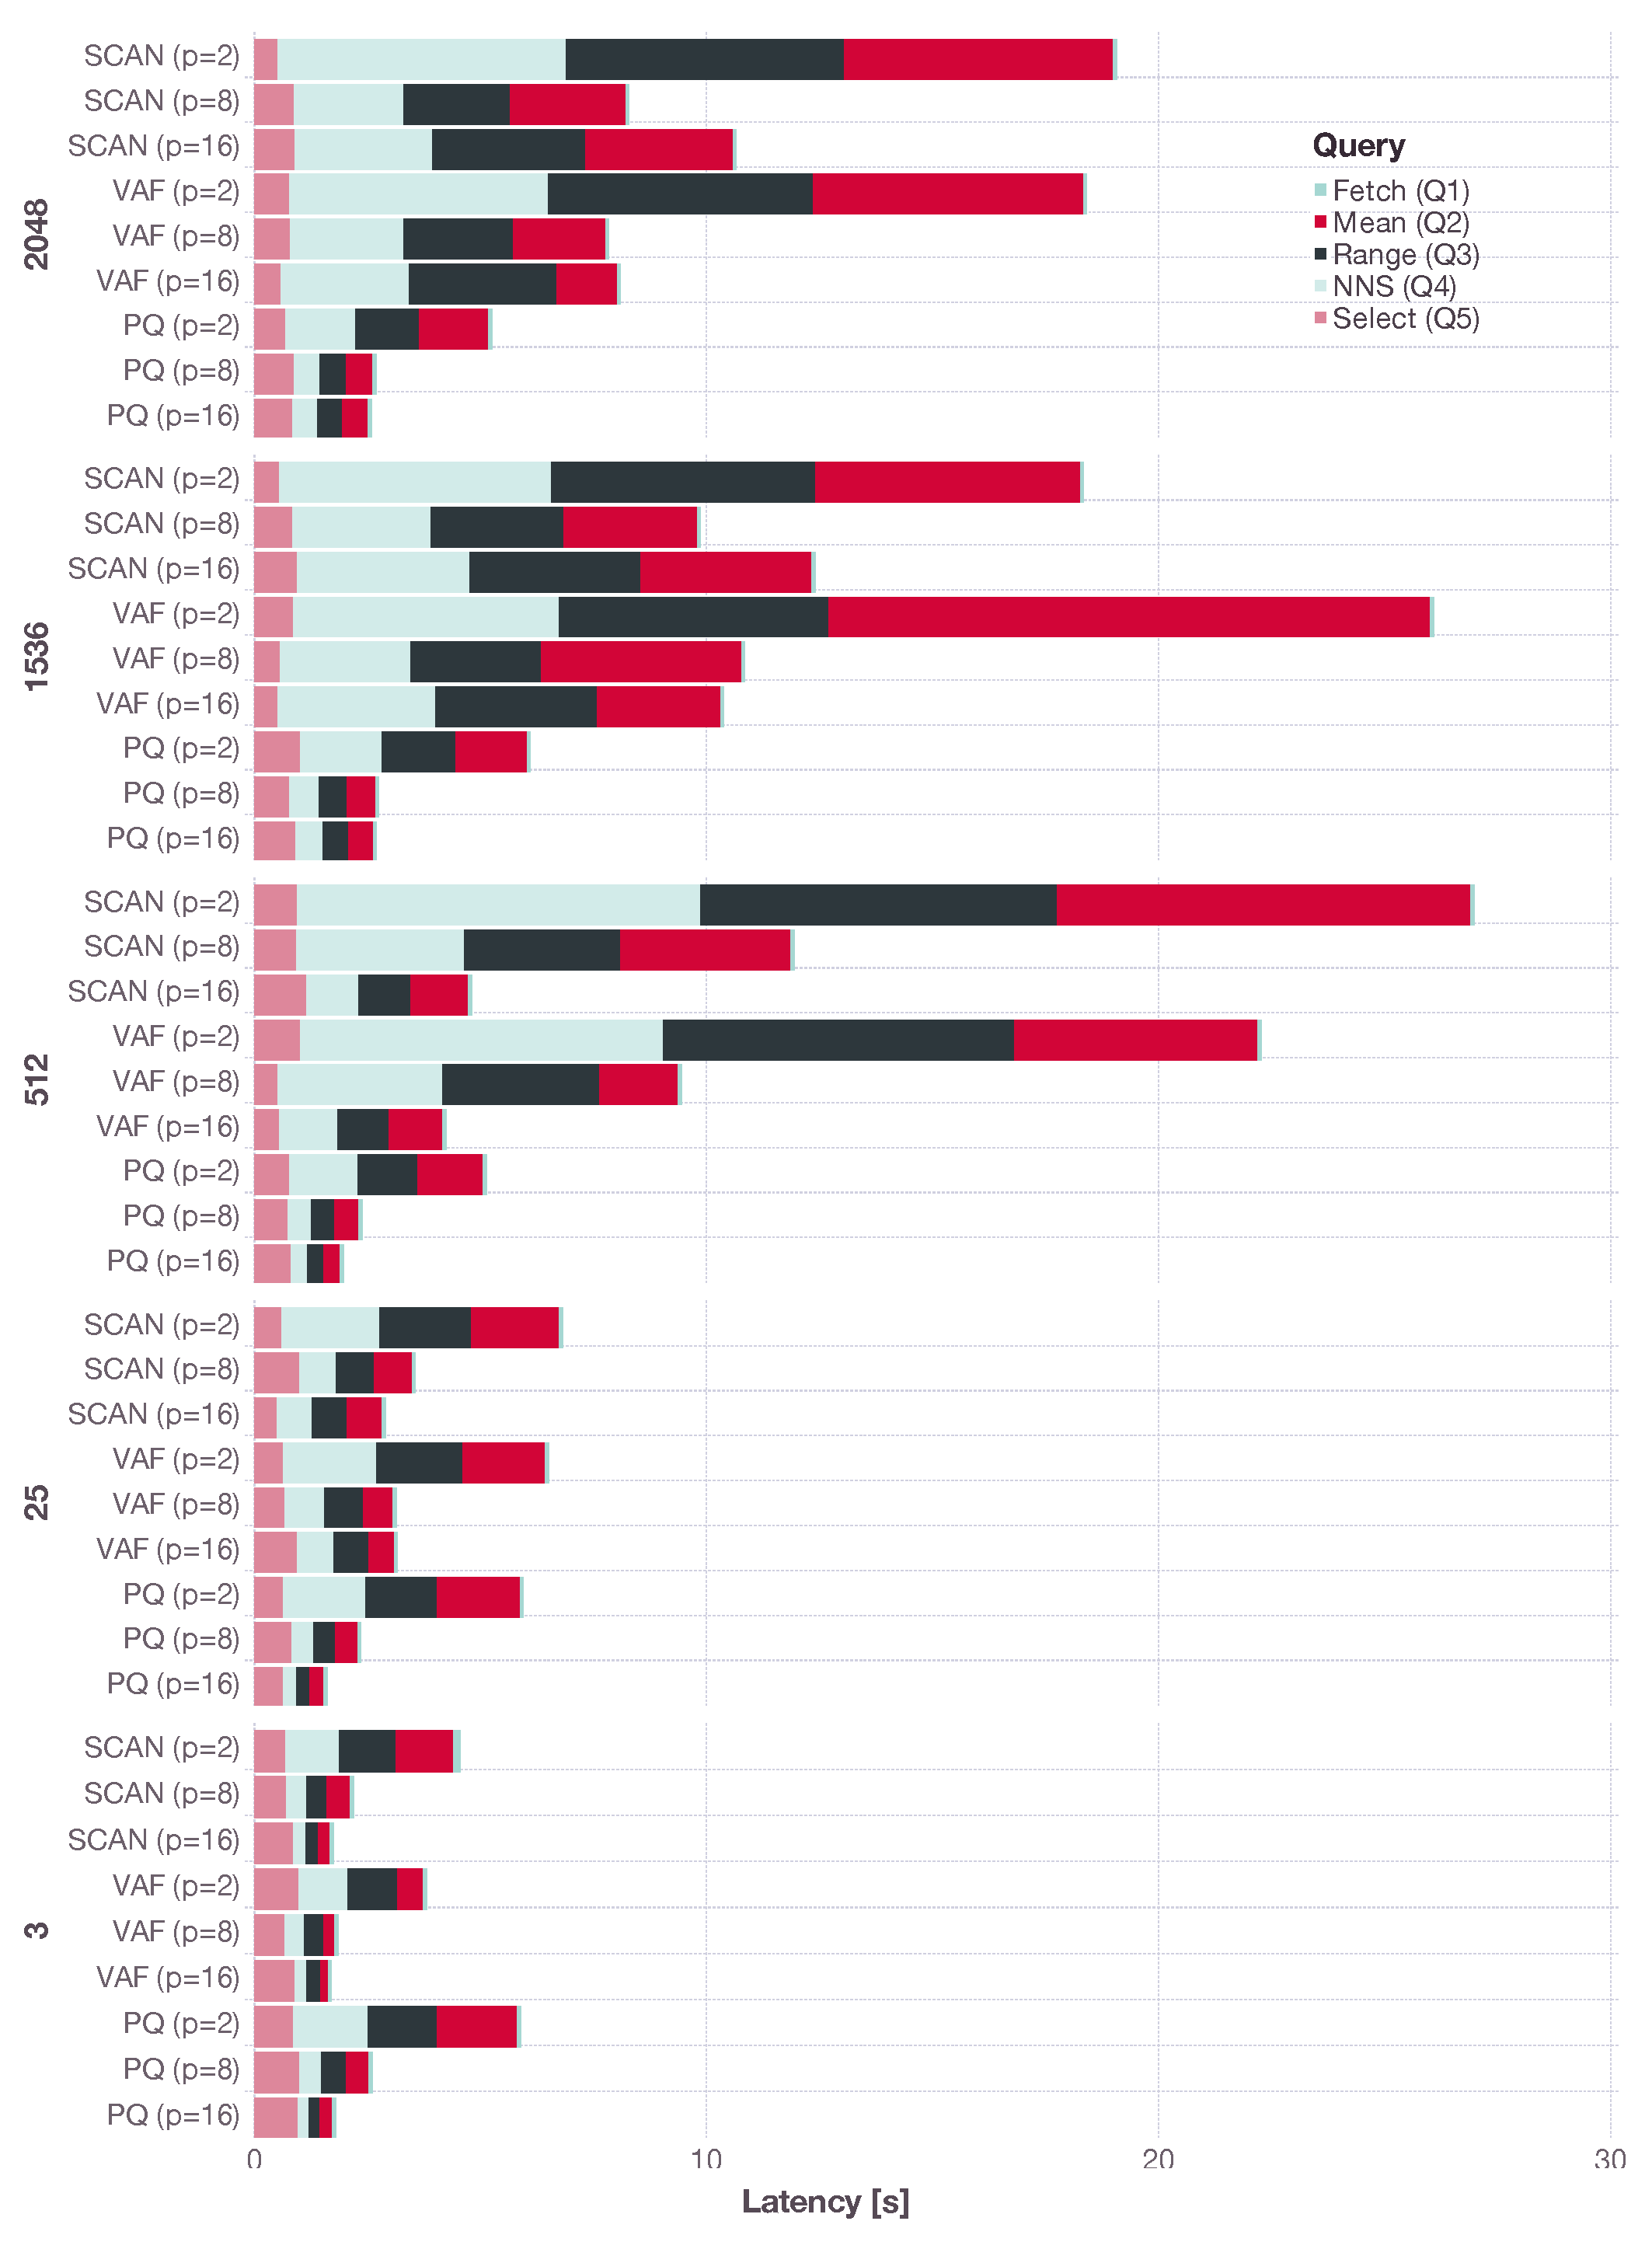
\includegraphics[width=\textwidth]{figures/analytics/analytics-cottontail-runtime}
    \caption {Latency in seconds (x-axis) on different entities using different access methods and levels of parallelisation (y-axis) for the analytics workloads during the first experiment. The individual queries Q1a-Q1e are highlighted in different colours. The use of the \acrshort{vaf} and \acrshort{pq} index was enforced using query hints.}
    \label{figure:analytics_cottontail_runtime}
\end{figure}

\begin{figure}[p]
    \centering
    \begin{subfigure}[b]{\textwidth}
        \centering
        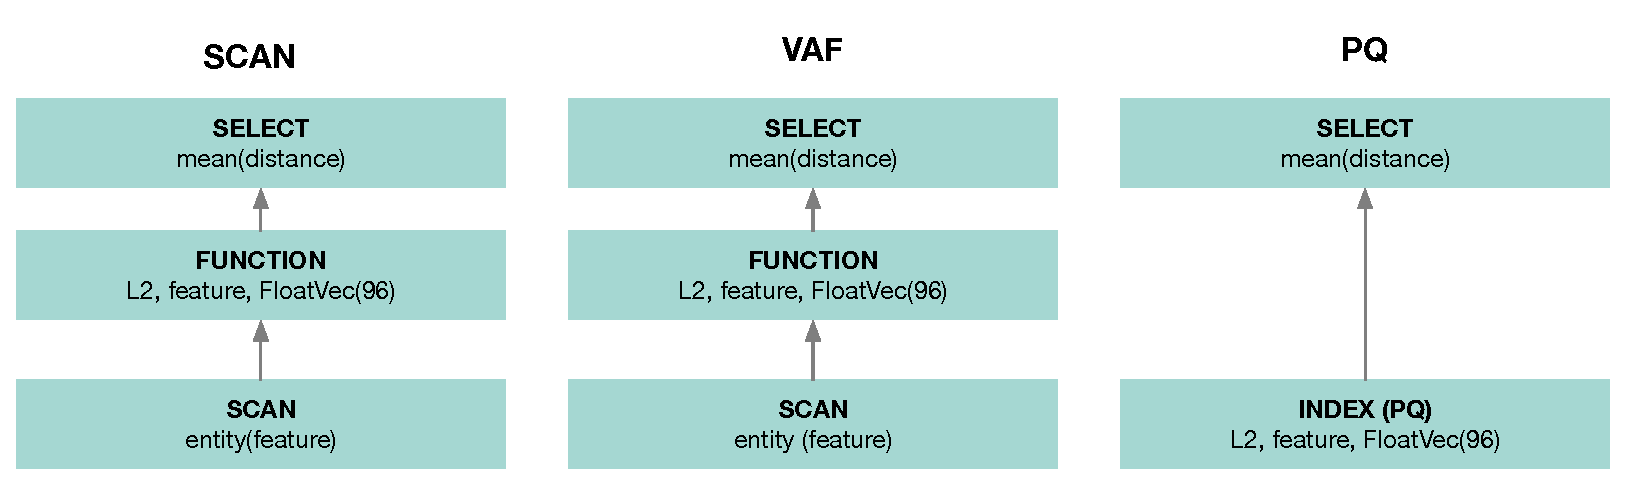
\includegraphics[width=\textwidth]{figures/analytics/query-plan-mean}
        \caption{Execution plans for mean query (Q1b)}
        \label{figure:cottontail_analytics_mean}
    \end{subfigure}
    \hfill
    \centering
    \begin{subfigure}[b]{\textwidth}
        \centering
        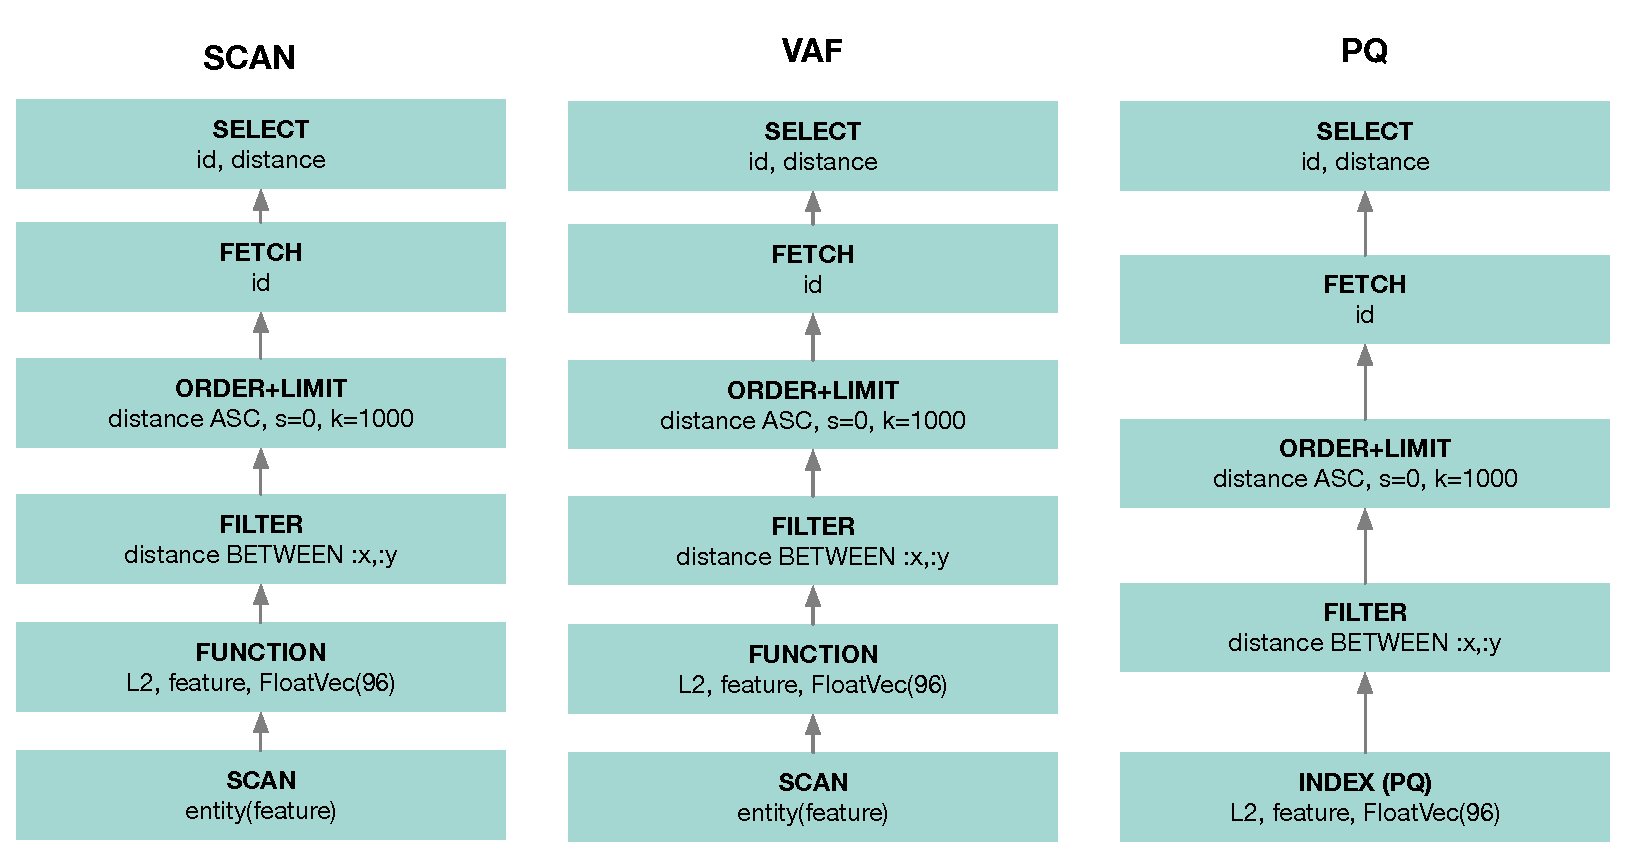
\includegraphics[width=\textwidth]{figures/analytics/query-plan-range}
        \caption{Execution plans for range query (Q1c)}
        \label{figure:cottontail_analytics_range}
    \end{subfigure}
    \hfill
    \centering
    \begin{subfigure}[b]{\textwidth}
        \centering
        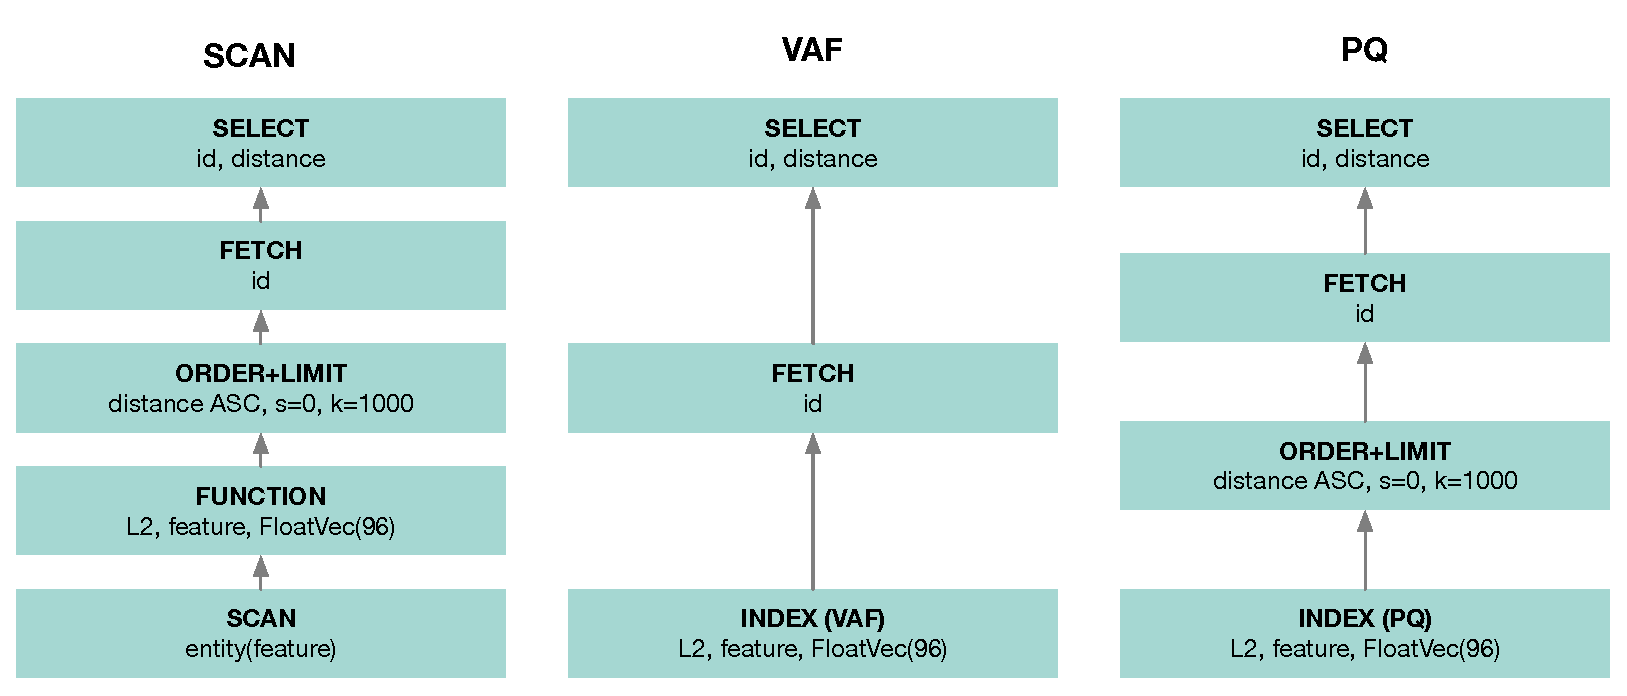
\includegraphics[width=\textwidth]{figures/analytics/query-plan-nns}
        \caption{Execution plans for \acrshort{nns} query (Q1d)}
        \label{figure:cottontail_analytics_nns}
    \end{subfigure}
    \caption{Execution plans produced by \cottontail{} for the mean (Q1b), range (Q1c) and \acrshort{nns} (Q1d) query workloads during the first experiment. The use of the \acrshort{vaf} and \acrshort{pq} index was enforced using query hints.}
    \label{figure:cottontail_analytics_plans}
\end{figure}

An aspect that we would like to draw the attention to is the influence of indexes: The Mean (Q1b), Range (Q1c) and \acrshort{nns} (Q1d) queries all seem to benefit from the PQ index, which, according to \Cref{figure:analytics_cottontail_runtime}, provides the lowest latency across all entities and for every degree of parallelisation. This is confirmed when cross-examining the query plans produced by \cottontail{}, which are listed in \Cref{figure:cottontail_analytics_plans}. The plans for the Q1b (\ref{figure:cottontail_analytics_mean}), Q1c (\ref{figure:cottontail_analytics_range}) and Q1d (\ref{figure:cottontail_analytics_nns}) indeed use the \acrshort{pq}, if the respective hint is present. This is possible because \acrshort{pq} can be used to perform a class 1 index replacement (see \Cref{definition:dfc_index_class_1}). 

However, the observed speed-up is traded for a non-negligible, negative impact on quality in terms of recall and n\acrshort{dcg}, as can be seen in \Cref{figure:cottontail_analytics_quality}. Slightly higher values for n\acrshort{dcg} provide us with an indication that mismatches occur further down in the ranking and may therefore be less relevant in practice. What is striking, though, is the very large spread for both recall and n\acrshort{dcg} across all collections, which indicates that the performance of an index is highly dependent on the concrete query vector and thus hard or even impossible to predict reliably. Furthermore, we can observe that the negative impact on quality seems to be larger for range (Q1c, \ref{figure:cottontail_analytics_quality_range}) than for \acrshort{nns} (Q1d, \ref{figure:cottontail_analytics_quality_nns}) queries for both recall and n\acrshort{dcg}. This can be explained by the distortion of the approximate distance as a side-effect of \acrshort{pq}, which has been reported by \cite{Jegou:2010Product} and which is obviously very relevant for range queries. We see this as a confirmation of our proposition, that quality metrics and statistics for the purpose of query planning should be obtained for a type of execution plan rather than globally per index (see \Cref{section:cost_model}). Additionally, we can observe that the same index configuration for \acrshort{pq} yields very different results for the different collections. Unfortunately, there does not seem to be an apparent correlation between the dimensionality and the quality of \acrshort{pq} index results, which implies that the quality depends on more than just the size of the vectors.

In contrast, the \acrshort{vaf} index can only provide speed-up for \acrshort{nns} queries (Q1d), since its use is limited to class 3 replacements (see \Cref{definition:dfc_index_class_3}) and the current implementation does not support range queries \footnote{ The latter is a limitation of our implementation and could be added, according to \cite{Weber:1998Va}}. Again, this is confirmed by the query plans shown in \Cref{figure:cottontail_analytics_plans}, where \cottontail{} resorts to a sequential scan in cases where the \acrshort{vaf} cannot be employed. The speed-up gained by using \acrshort{vaf} seems rather small and it is directly related to the efficiency of the filtering. Over the different runs, we observed \acrshort{vaf} filter efficiency values of between $80\%$ and $99\%$. Again, there seems to be no apparent connection between dimensionality and the effectiveness of the filtering step.

\begin{figure}[tb]
    \centering
    \begin{subfigure}[b]{\textwidth}
        \centering
        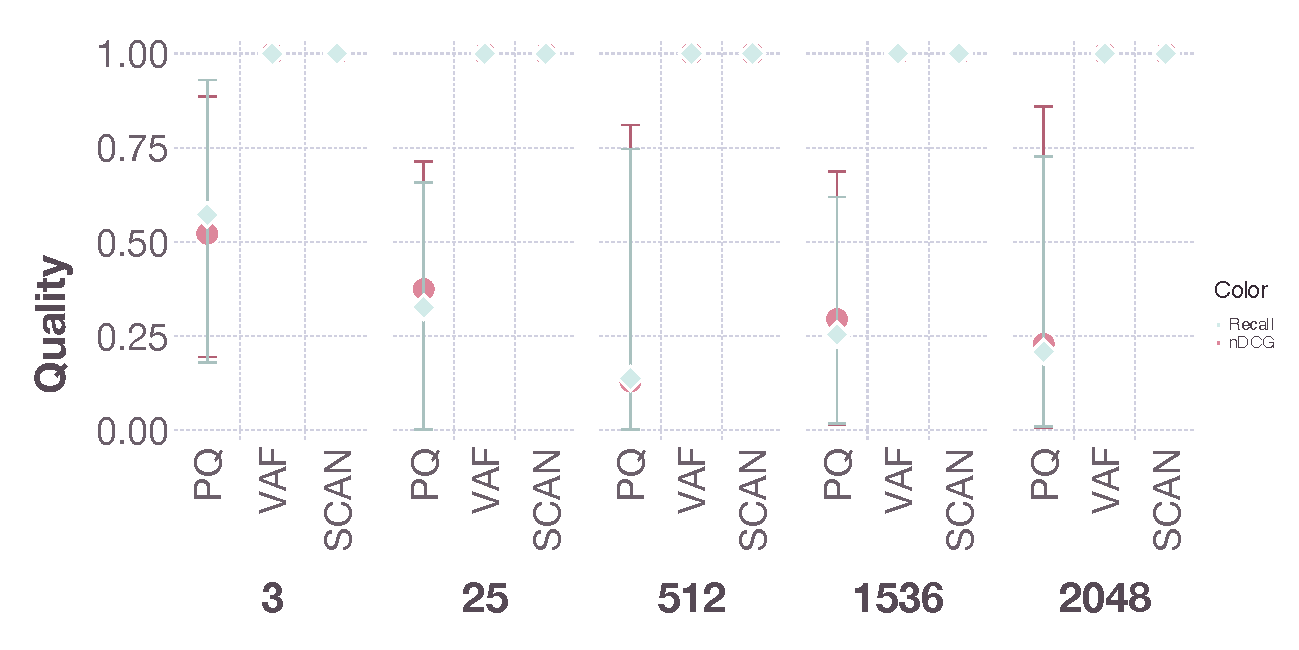
\includegraphics[width=\textwidth]{figures/analytics/analytics-cottontail-quality-range}
        \caption{Quality for range query (Q1c)}
        \label{figure:cottontail_analytics_quality_range}
    \end{subfigure}
    \hfill
    \centering
    \begin{subfigure}[b]{\textwidth}
        \centering
        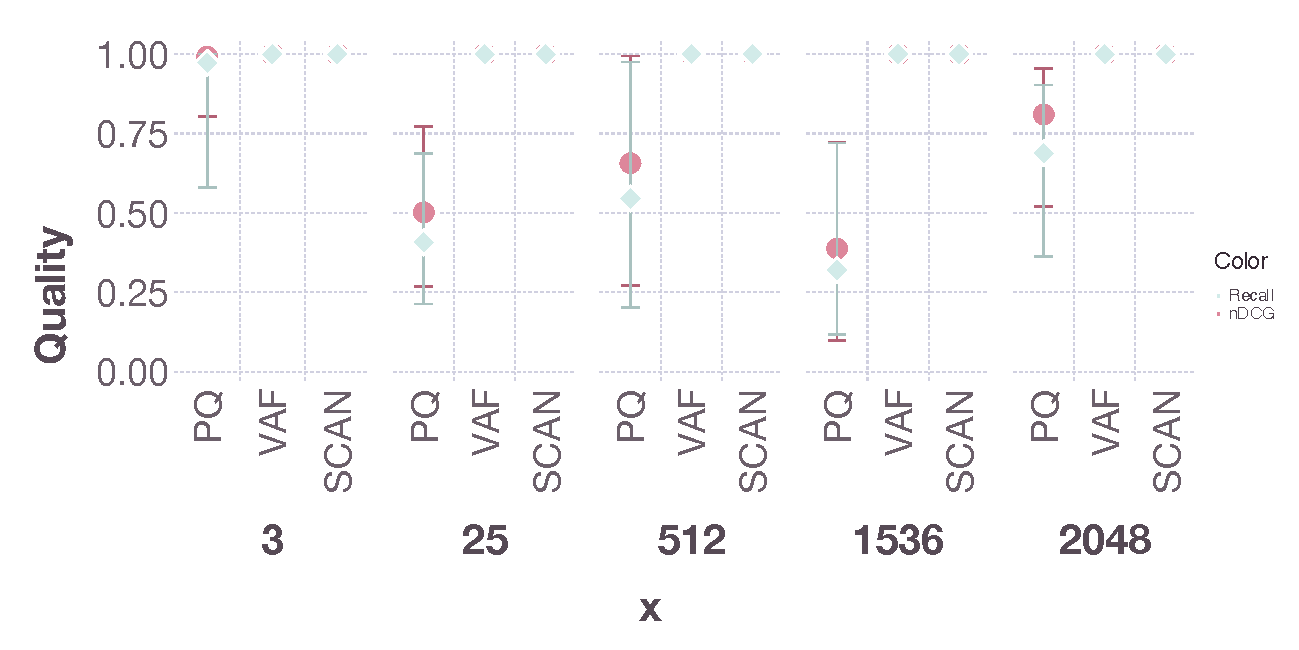
\includegraphics[width=\textwidth]{figures/analytics/analytics-cottontail-quality-nns}
        \caption{Quality for \acrshort{nns} query (Q1d)}
        \label{figure:cottontail_analytics_quality_nns}
    \end{subfigure}
    \caption{Quality of results (x-axis) in terms of recall (mint) and \acrshort{dcg} (red) on different entities using different access methods (y-axis) for the range (Q1c) and \acrshort{nns} (Q1d) query workloads during the first experiment. The use of the \acrshort{vaf} and \acrshort{pq} index was enforced using query hints.}
    \label{figure:cottontail_analytics_quality}
\end{figure}

We must assume, that the quality of all the tested index structures can be fine-tuned by chosing appropriate values for the hyperparameters. Since these values seem to depend on a multitude of factors (e.g., collection size, structure of the data, dimensionality), this may not be a straightforward undertaking. However, learning an optimal set of hyperparameters for a given collection and index  could be an interesting research direction for the future, very similar to learned index structures proposed by \cite{Kraska:2018Case}.

\subsection{Experiment 2: Influence of Cost Policy}
\label{section:cost_model_evaluation}

So far, we have forced \cottontail{} into using one index over another by providing query hints that make an explicit choice. For this second experiment, we delegate the decision to \cottontail{} and observe how changing parameters in the cost policy influence plan selection. The idea behind the cost policies was explained in \Cref{section:cost_model}. Basically, they assign weight to the parameters of the cost model -- the cost of IO, CPU, memory use and reduction in quality -- and can be used to steer the planner's behaviour depending on the use-case. For the experiment, we fixed the values of $w_{\mathtt{CPU}} = 0.3$, $w_{\mathtt{IO}} = 0.6$ and $ w_{\mathtt{MEM}} = 0.1$ respectively (\cottontail{}'s default values) via the respective query hint. We then used the \texttt{EXPLAIN} endpoint to generate and print the execution plans as we increased the weight of the quality parameter $w_{\mathtt{Q}}$ from $0.1$ to $0.9$ in steps of $0.1$. The results are depicted separately for the mean (Q1b, \ref{figure:cottontail_analytics_cost_mean}), range (Q1c, \ref{figure:cottontail_analytics_cost_range}) and \acrshort{nns} (Q1d, \ref{figure:cottontail_analytics_cost_nns}) queries, for which we plot the scores and the ranking assigned to the individual plans by \cottontail{}'s query planner. Furthermore, we visualise all query execution plans that appear in the top three ranks at some point.

\begin{figure}[tb]
    \centering
    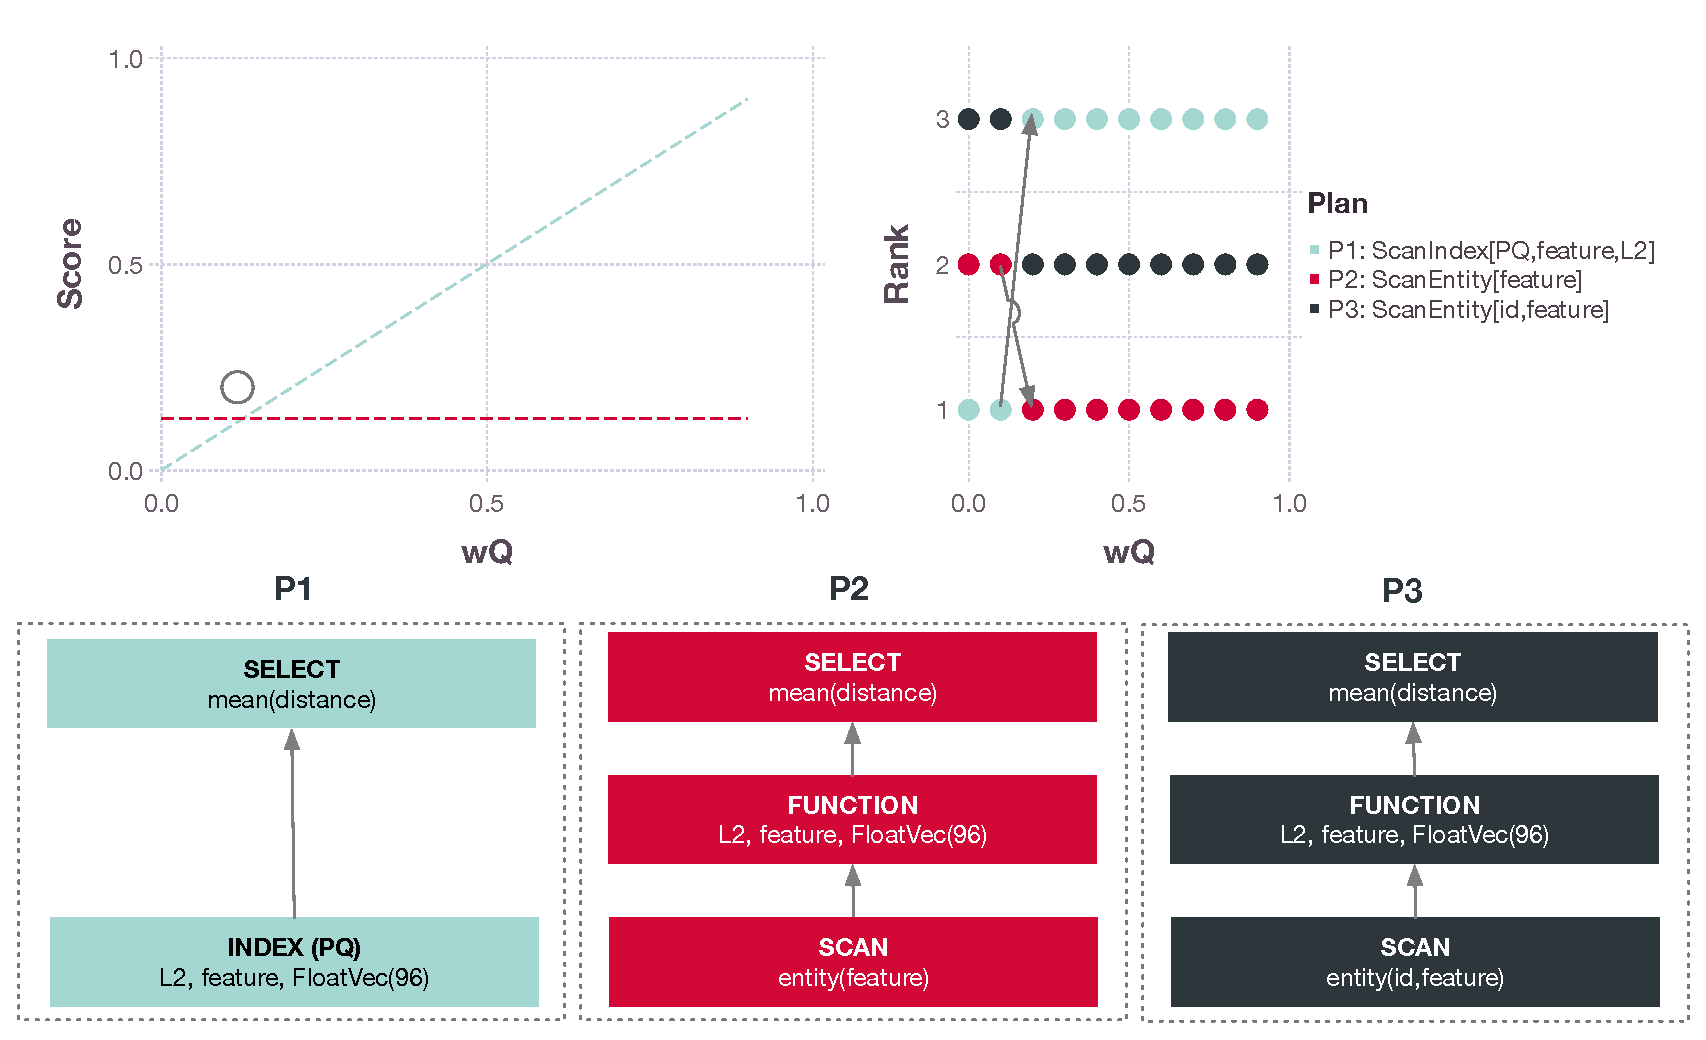
\includegraphics[width=\textwidth]{figures/analytics/analytics-cottontail-cost-mean-annotated}
    \caption{Score and rank of different query plan options for the mean query (Q1b). The prefered option for $w_{\texttt{Q}} = 0.0$ involves the scan of a \acrshort{pq} index. As $w_{\texttt{Q}}$ goes up, the cost of impaired quality increases and a full entity scan ($P_2$) takes over, since none of the available indexes can satisfy the query. The scores for $P_2$ and $P_3$ do not depend on the quality parameter and incur almost the same cost, with $P_2$ being the less expensive variant.}
    \label{figure:cottontail_analytics_cost_mean}
\end{figure}

For Q1b (\Cref{figure:cottontail_analytics_cost_mean}) we see that at least three different options exists and that by default, i.e., for $w_{\mathtt{Q}} = 0.0$, the option involving the \acrshort{pq} index ($P_1$) is favoured. This is consistent with the findings from our first benchmark, where we demonstrated that \acrshort{pq} is the fastest of the available options. As long as the quality weight parameter is low ($w_{\mathtt{Q}} \in [0.1, 0.2]$), $P_1$ remains the plan with the lowest score and thus the selected candidate. As $w_Q$ increases, the score of $P_1$ increases as well and it moves up in the ranking and plan $P_2$, which involves a full table scan, takes over the lead. The two alternatives $P_2$ and $P_3$ are almost equivalent with the only difference that $P_3$ includes the \texttt{id} column in the initial scan, which is not required to calculate the mean and can therefore be optimised out (the application the deferral rules described in \Cref{section:cottontail_query_planner}). Consequently, $P_3$ is slightly more expensive and $P_2$ is selected instead. 

\begin{figure}[p]
    \centering
    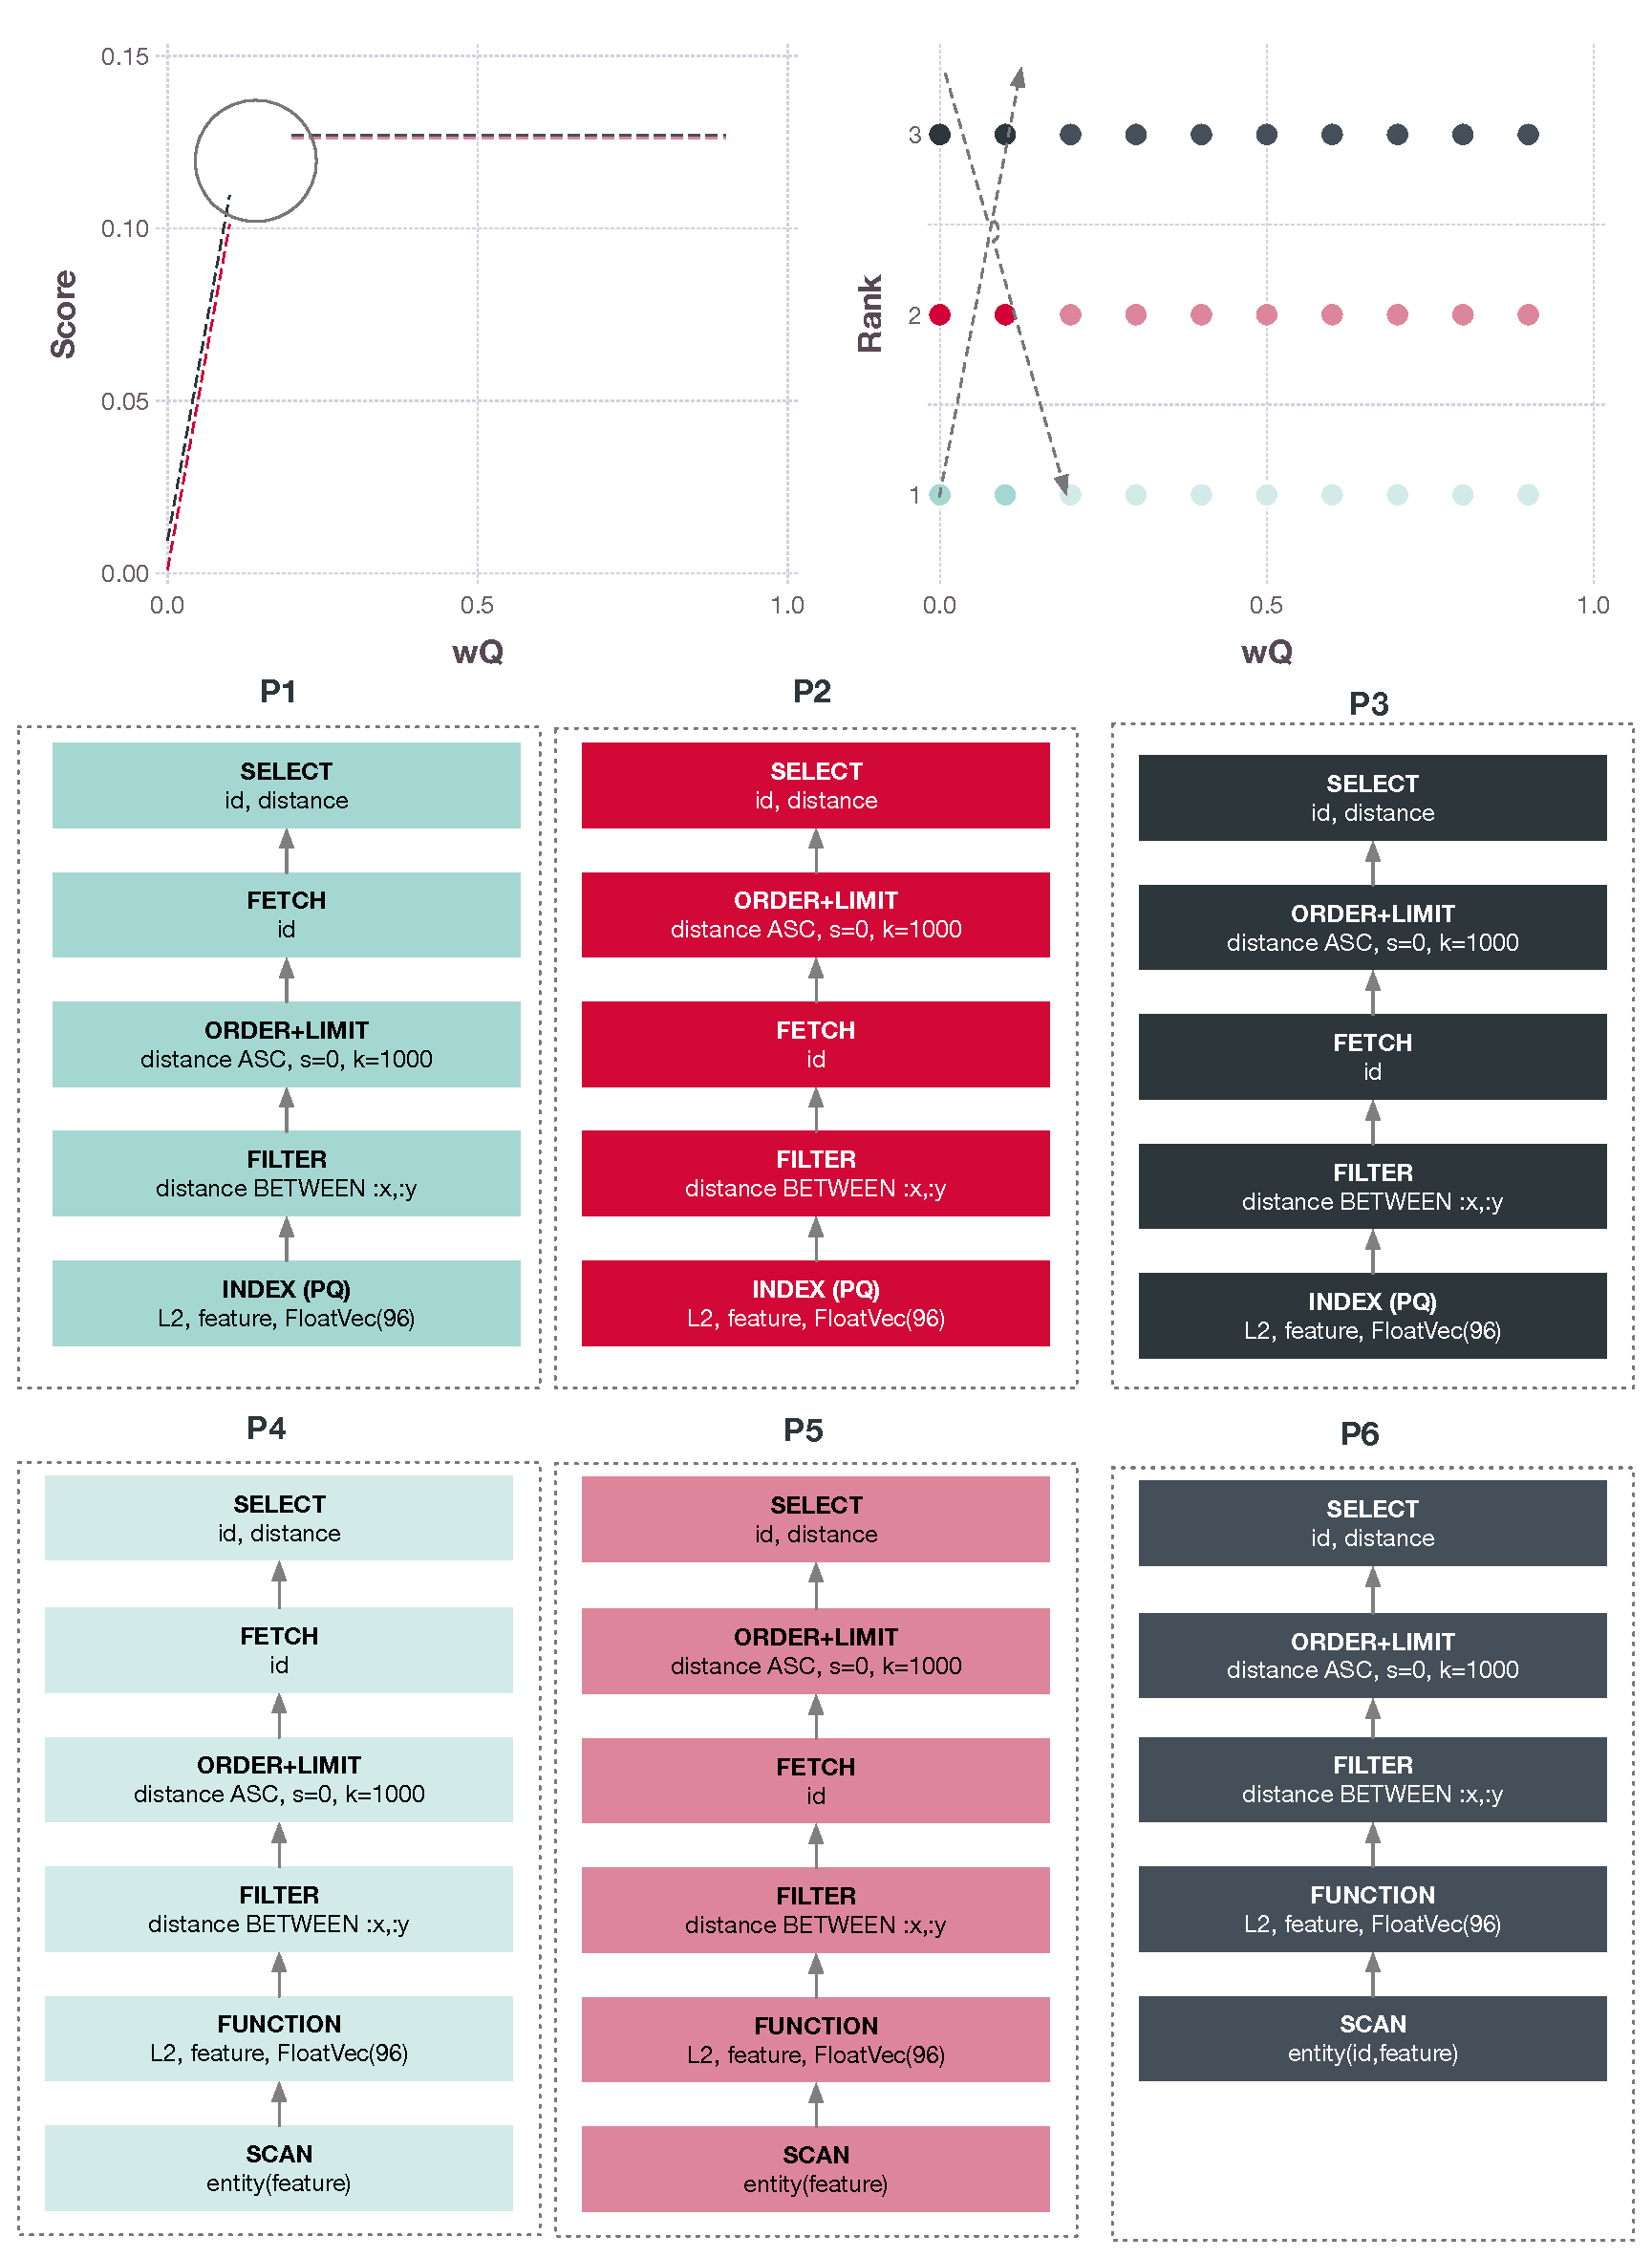
\includegraphics[width=\textwidth]{figures/analytics/analytics-cottontail-cost-range-annotated}
    \caption{Score and rank of different query plan options for the range query (Q1c). The prefered option for $w_{\texttt{Q}} = 0.0$ involves the scan of a \acrshort{pq} index. As $w_{\texttt{Q}}$ goes up, the cost of impaired quality increases and a full entity scan takes over, since none of the available indexes can satisfy the query. The scores for $P_4$ through $P_6$ do not depend on the quality parameter and incur almost the same cost, with $P_4$ being the least expensive.}
    \label{figure:cottontail_analytics_cost_range}
\end{figure}

\begin{figure}[p]
    \centering
    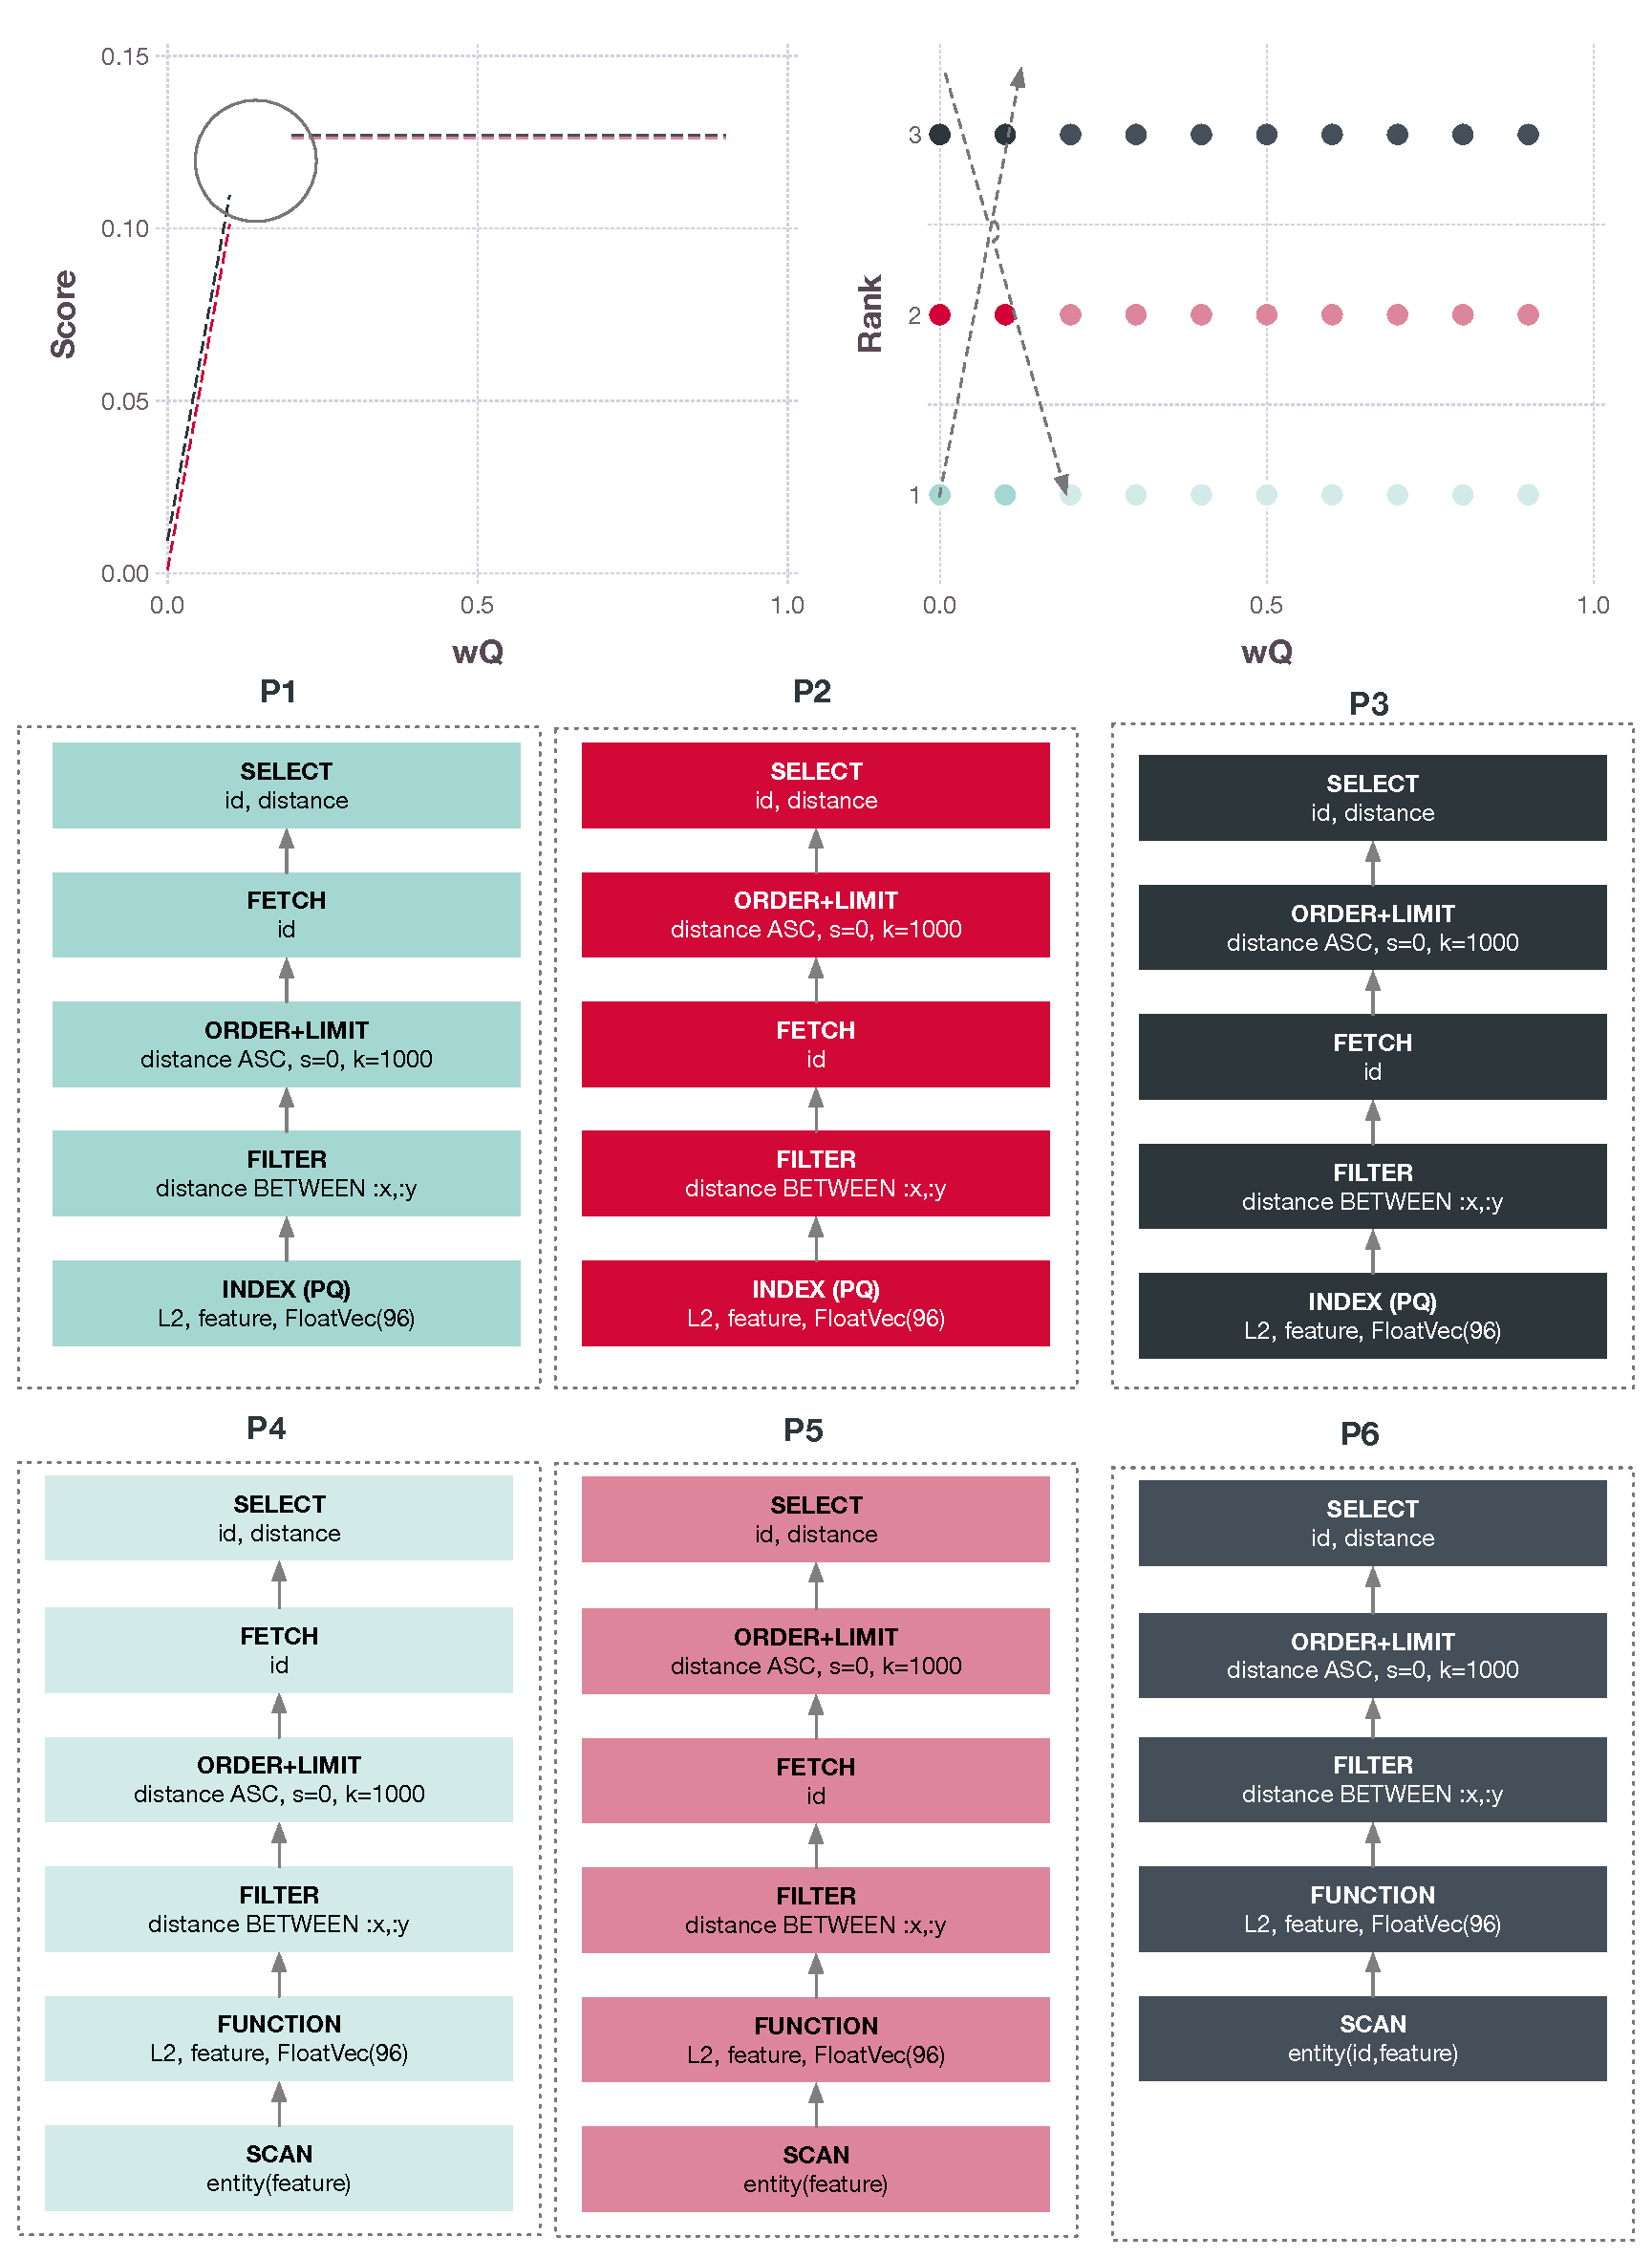
\includegraphics[width=\textwidth]{figures/analytics/analytics-cottontail-cost-nns-annotated}
    \caption{Score and rank of different query plans options for the \acrshort{nns} query (Q1d). The prefered option for $w_{\texttt{Q}} = 0.0$ involves the scan of a \acrshort{pq} index. As $w_{\texttt{Q}}$ goes up, the cost of impaired quality increases and a \acrshort{vaf} index scan ($P_3$) takes over, which can also satisfy \acrshort{nns} queries. Since \acrshort{vaf} does not incur a quality cost, it remains the favoured option.}
    \label{figure:cottontail_analytics_cost_nns}
\end{figure}

A very similary behaviour can be observed for Q1c (\Cref{figure:cottontail_analytics_cost_range}). Over the course of the measurements, six options appear in the top $3$ ranks. Again, we start with  $w_{\mathtt{Q}} = 0.0$, where $P_1$ is the fastest option and again, it involves a scan of the \acrshort{pq} index. $P_2$ and $P_3$ are different variants involving the same index scan but using different intermediate operations and therefore differ in the fetching of required columns and sort algorithms (application of the deferral and implementations rules described in \Cref{section:cottontail_query_planner}). As $w_Q$ increases, $P_1$, $P_2$ and $P_3$ disappear from the top $3$ ranks, since all three plans use the same index and therefore result in impaired quality. $P4$ -- which is the query plan involving the evaluation of a full entity scan -- takes over and keeps the lowest rank. Again, $P5$ and $P6$ are less optimal variants of $P4$ and are therefore not considered.

For both Q1b and Q1c using \acrshort{pq} or a full entity scan were the only available options due to the constraints discussed in \Cref{section:dfc_and_indexes}. For Q1d (\Cref{figure:cottontail_analytics_cost_nns}) we see a third option appear, which is the use of a \acrshort{vaf} index ($P3$). As $w_{\mathtt{Q}}$ exceeds $0.1$, the scan of the \acrshort{vaf} index becomes the prefered candidate and $P_1$ and $P_2$ become the second and third options. As $w_{\mathtt{Q}}$ moves beyond $0.2$, $P_1$ and $P_2$ disappear from the top 3 and the entity scan becomes the prefered alternative to the \acrshort{vaf} index scan. However, since the \acrshort{vaf} index does not incur a quality cost, it remains the favoured option.

\newpage

\subsection{Benchmark 3: Influence of Optimisation}
We have demonstrated in the first experiment, that high-dimensional index selection has a considerable impact on query execution performance. However, as described in \Cref{chapter:cottontaildb}, in addition to selecting indexes, the query planner also performs other optimisations of the plan before executing it. For this experiment, we bypassed plan optimisation completely and observed the execution time for an unoptimised plan -- which is a naive implementation of the canoncial operator tree. All experiments were performed with parallelisation switched off, i.e., every query was executed in a single thread. The results are depicted in \Cref{figure:cottontail_analytics_optimisation}.

\begin{figure}[p]
    \centering
    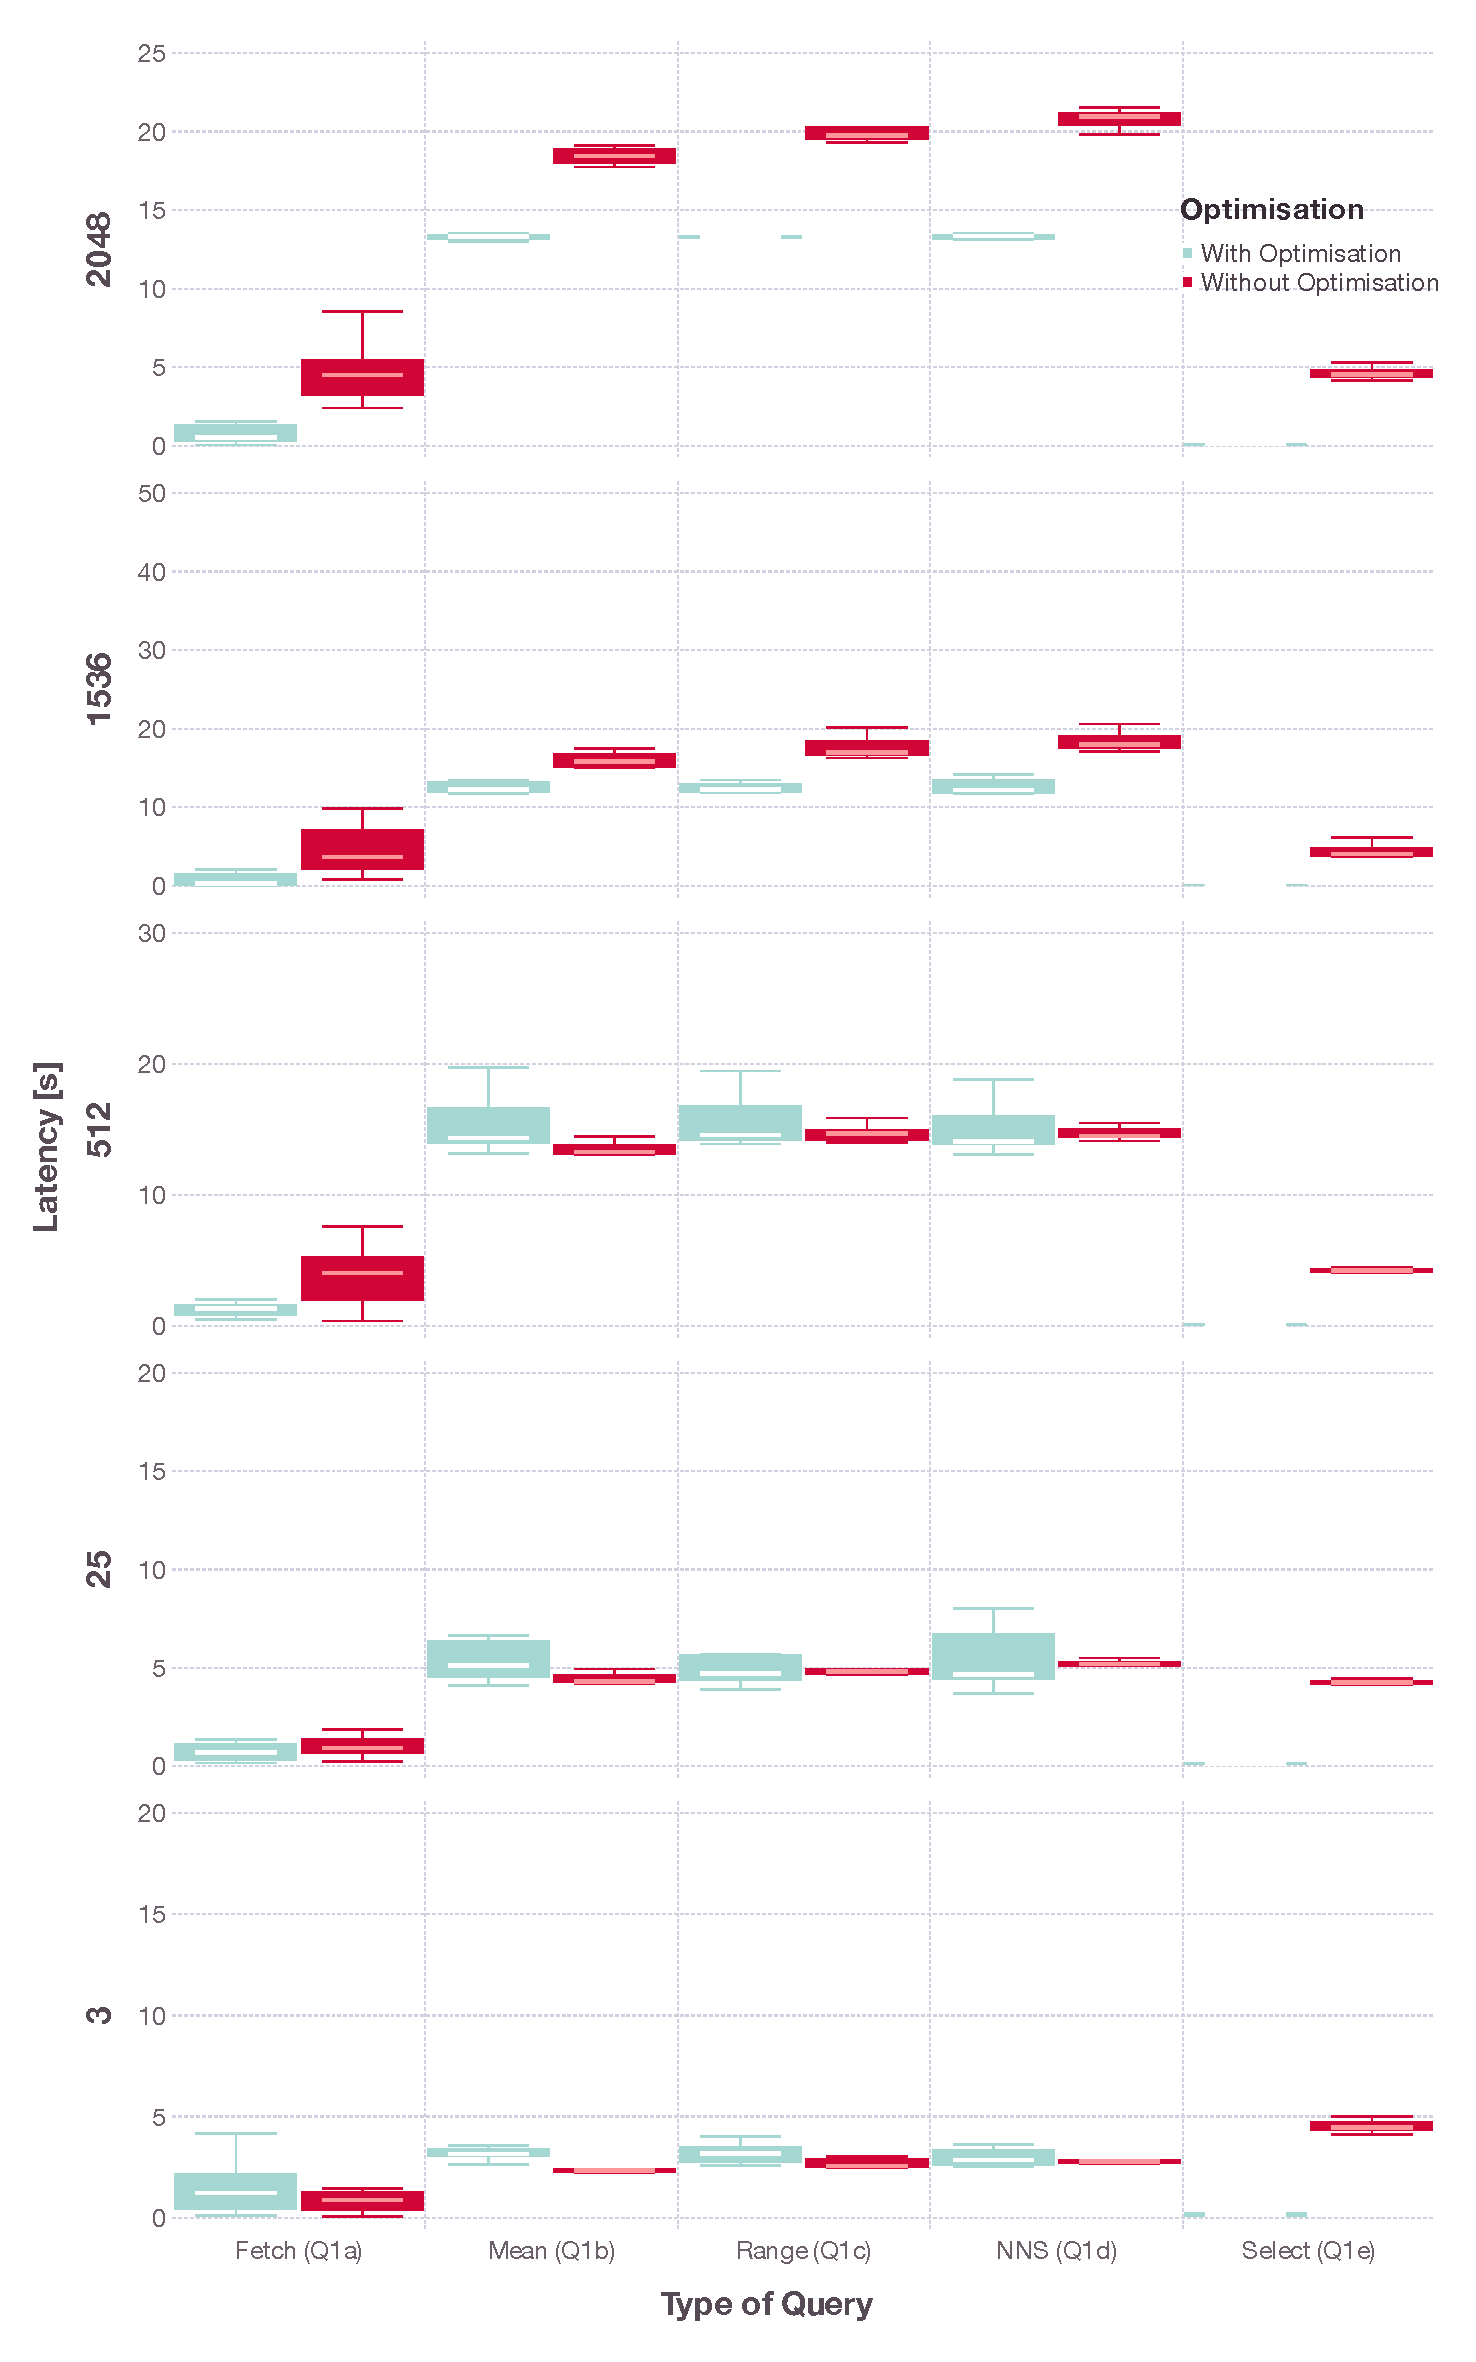
\includegraphics[width=\textwidth]{figures/analytics/analytics-cottontail-optimisation-runtime}
    \caption{Latency in seconds on different collections (y-axis) for the query workloads Q1a through Q1e (x-axis) with (mint) and without (red) query optimisation.}
    \label{figure:cottontail_analytics_optimisation}
\end{figure}

We can see from this graph, that optimisation seems to have a larger effect on latency for proximity based queries (Q1b to Q1d) involving high-dimensional vectors than it does for low dimensional ones. However, optimisation also seems to introduce a larger variance in latency, making it less predictable. Both effects can be attributed to the column-access deferral optimisation rule, which pushes access to columns that are not required for query execution up in the tree until after a ($s,k$-)selection has been executed. The idea is to reduce or even avoid access to data that is not needed and therefore the number of IO operations. This optimisation seems to be highly relevant for large vectors but it diminishes as dimensionality decreases. We suspect that the page cache, which -- given the huge amount of memory available -- can keep many of the requested pages in memory, is responsible for this behaviour. When larger entities are being scanned, the cache becomes more saturated and the likelihood of a cache miss becomes higher resulting in a higher, overall latency. This effect is of course amplified if more than one column is being scanned (unoptimised). The higher variance can be explained by the fetch-opertion, which equates to random access and is thus less predictable than the linear scan, for which mechanisms like pre-fetching can be employed.

As a second observation, we see that optimisation consistently benefits the Select (Q1e) query, where we load segment entries that match the preceding query results. The exaplanation here is as simple as unexciting: The select query (Q1e) benefits from a $B^{+}$-tree index scan in the optimised case, while the unoptimised case uses a full entity scan.
 
Last but not least, we see that the impact of optimisation is slight larger for range (Q1c) and \acrshort{nns} (Q1d) queries than it is for the mean query. This can be attributed to a second optimisation, which combines the sorting and limiting used for Q1c and Q1d into a single step that uses a specialised heap data structure. This sort algorithm can be executed more efficiently and uses less memory than the naive sorting. However, since memory is effectively not a constraint in our setting, we expect the impact to be even larger for setups that do not exhibit the same amount of memory and must therefore resort to on-disk sorting.

\newpage

\section{Large-Scale Similarity Search}
This series of measurements is a direct comparison between Milvus and \cottontail{} and is about mere performance. We execute all queries on prepared shards of the Deep1B \cite{Babenko:2016Efficient} dataset ($d=96$) with $k=1000$ using different execution strategies and compare the obtained metrics. The shards contain 5 million, 10 million, 100 million and 1 billion $96$-dimensional \texttt{float} vectors and are stored in dedicated collections (Milvus) or entities (\cottontail). The Psudo-\acrshort{sql} of the three types of queries is listed in \Cref{listing:big_nns_query}:
\begin{enumerate*}[label=(\roman*)]
    \item A simple \acrshort{nns} query that only returns the primary key and the distance (Q2a),
    \item a \acrshort{nns} query that additionaly returns the query vector (Q2b),
    \item a \acrshort{nns} query with a Boolean filter (Q2c, hybrid query in Milvus terminology).
\end{enumerate*} We use the query vectors provided with the Deep1B dataset and establish a groundtruth by executing a brute-force search.

\begin{lstlisting}[language=SQL, caption={Pseudo-SQL of the queries executed for this measurement.}, label=listing:big_nns_query, numbers=none]
    /* Q2a: Simple NNS without feature vectors. */
    select id, euclidean(feature, <query>) as dst from <collection> order by dst limit 1000
    
    /* Q2b: NSS that returns feature vectors. */
    select id, feature, euclidean(feature, <query>) as dst from <collection> order by dst limit 1000

    /* Q2c: Hybrid query without feature vector. */
    select id, euclidean(feature, <query>) as dst from <collection> where category = <category> order by dst limit 1000
\end{lstlisting}

\subsection{\cottontail}
\label{section:evaluation_bignns_cottontail}
For this benchmark, we prepared a selection of indexes on the respective entities in \cottontail{}: Two variants of a \acrshort{pq} index, once organised as a list for exhaustive search ($8$ subspaces, $256$ centroids) and once organised as an inverted list for approximate search ($8$ subspaces, $256$ centroids and $256$ coarse centroids) and a \acrshort{vaf} index. Furthermore, we created a $B^{+}$-Tree index on the column \texttt{categories}, which we expect to be beneficial for Boolean search. We again use query hints to nudge \cottontail{} into using certain high-dimensional index structures so as to be able to compare the different query execution strategies. Accross all workloads, we compare the performance of four different types: Sequential scan and the scan of the \acrshort{vaf} and the (IVF-)\acrshort{pq} indexes.

\begin{landscape}
    \begin{figure}[p]
        \centering
        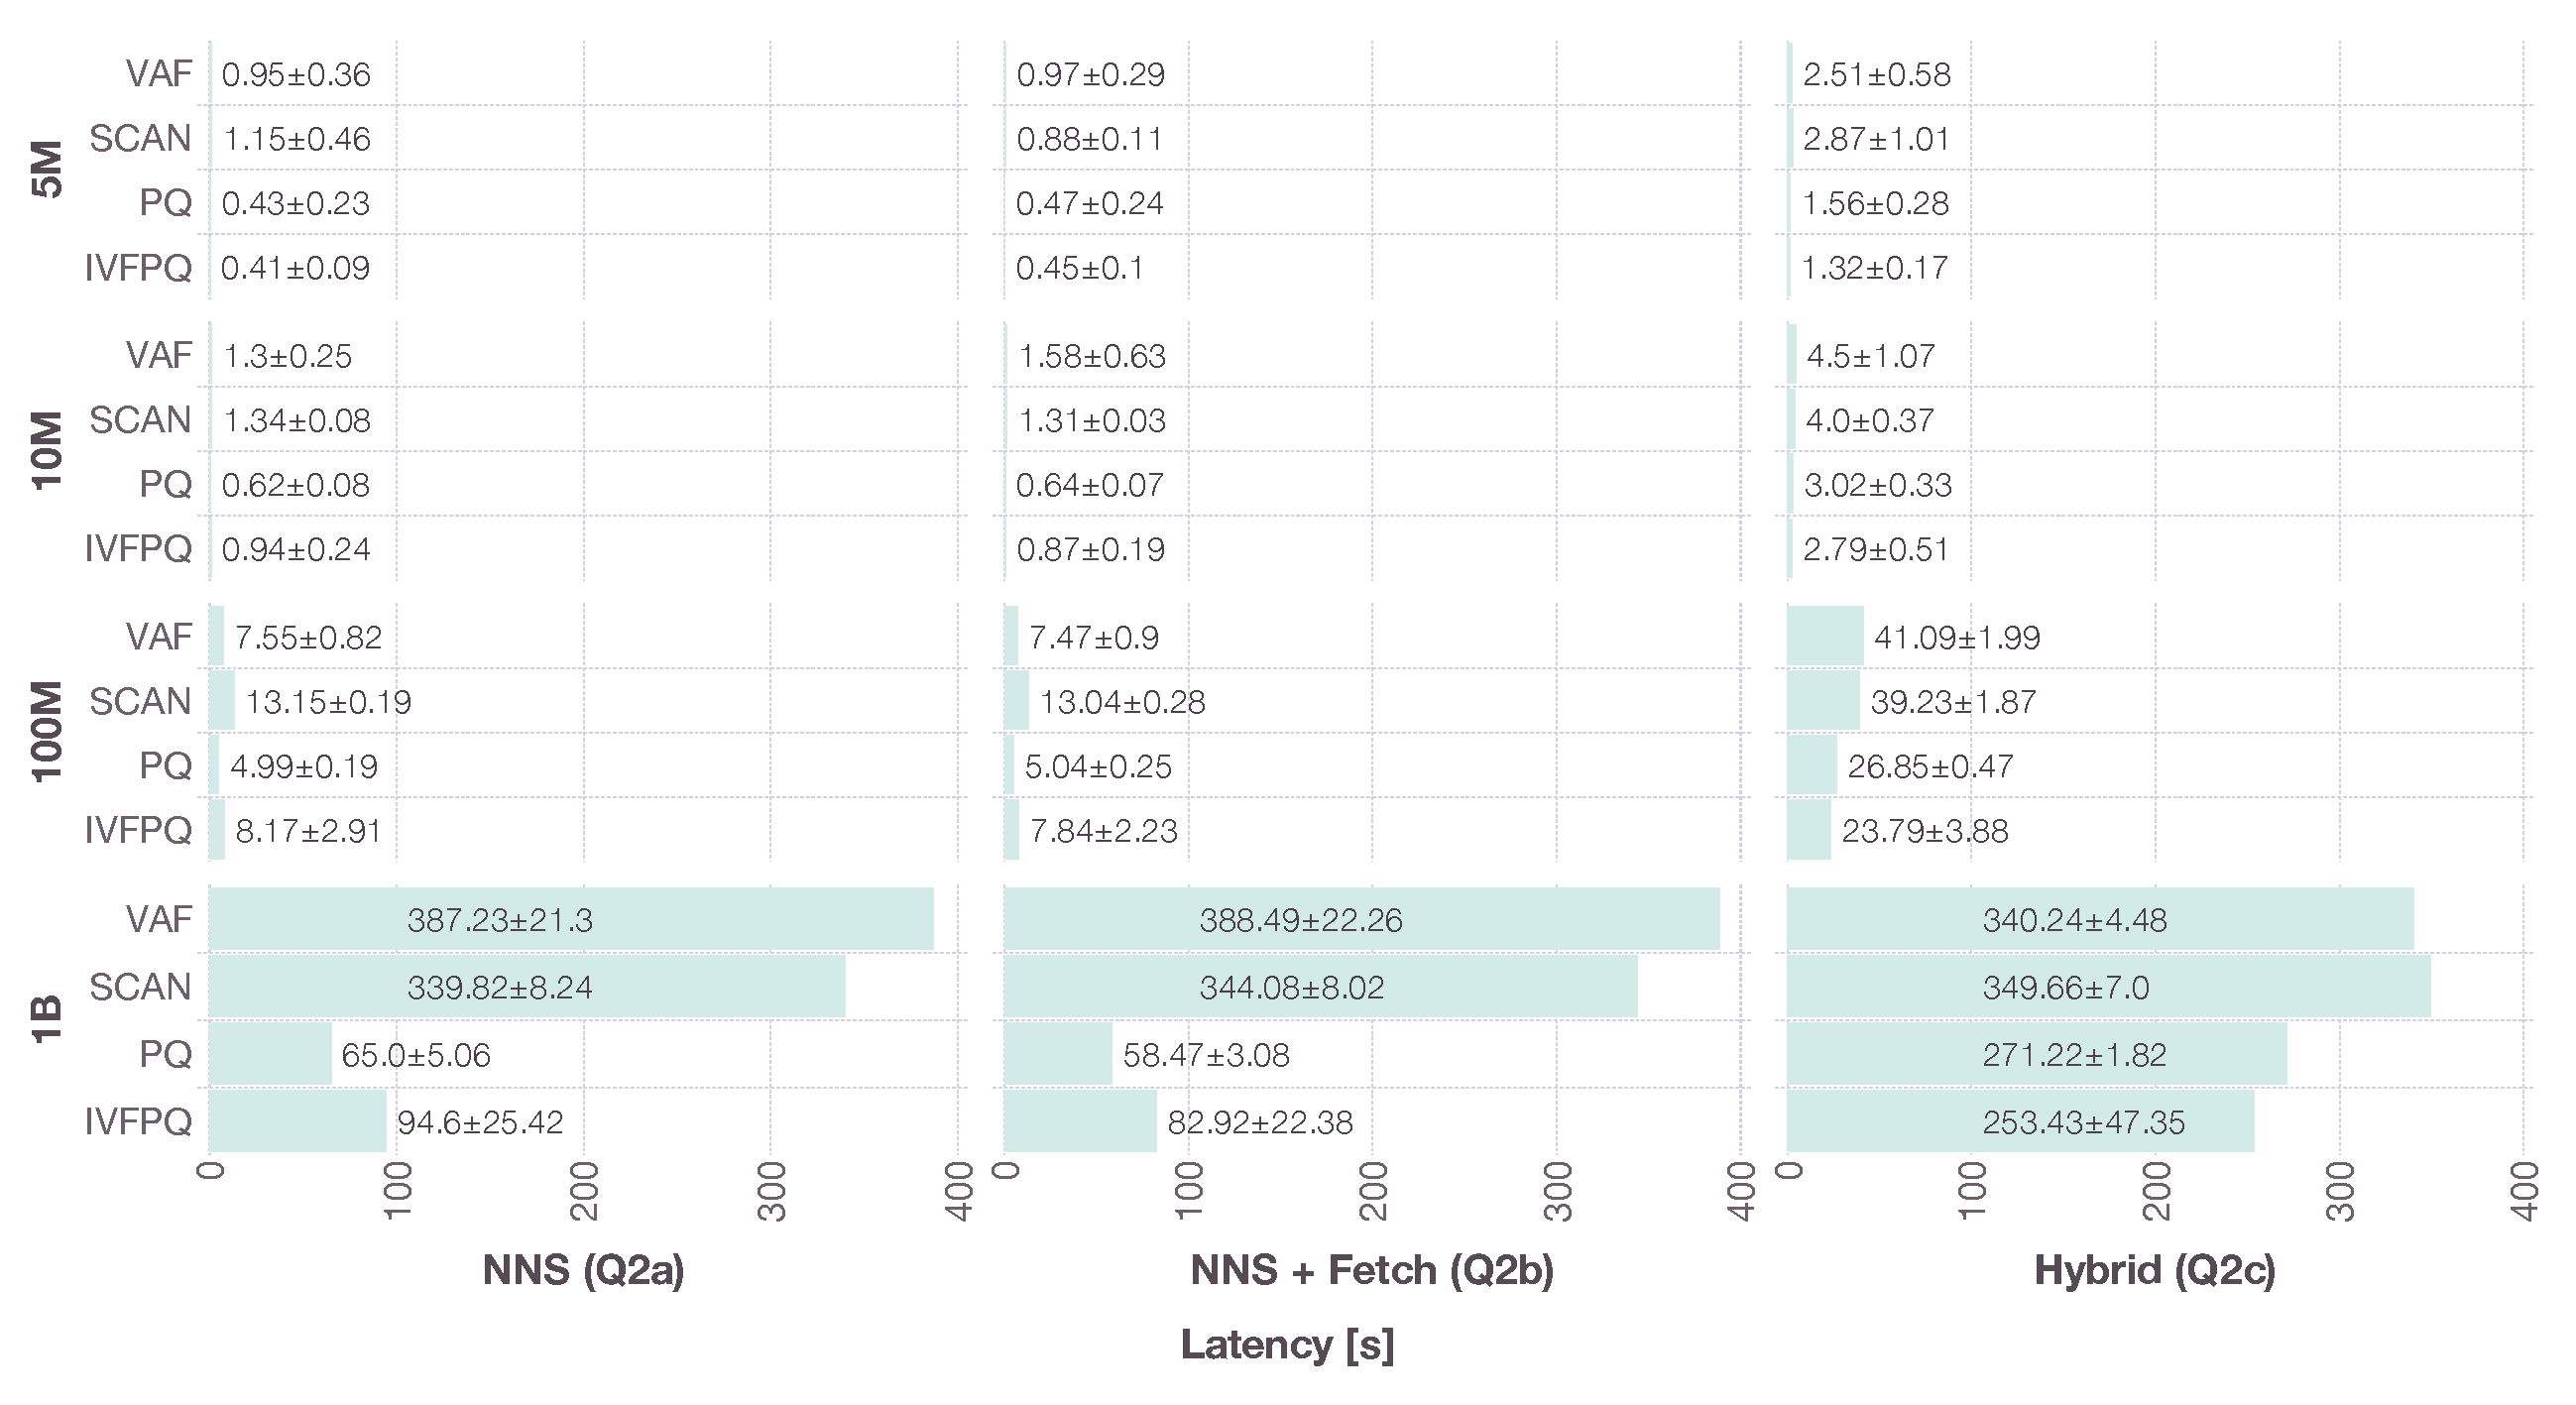
\includegraphics[width=1.55\textwidth]{figures/bignns/cottontail/bignns-cottontail-runtime}
        \caption {\cottontail{}'s latency in seconds for different workloads (x-axis) on different shards of the Deep 1B data set using different execution strategies (y-axis).}
        \label{figure:cottontail_runtime}
    \end{figure}
\end{landscape}

In our first experiment, we executed the simple \acrshort{nns} workload (Q2a). The results are depicted in \Cref{figure:cottontail_runtime}. Brute-force search took between $0.95 \pm 0.36 \, \si{\second}$ (5 million) and $339.82 \pm 8.24 \, \si{\second}$ (1 billion). We can observe, that the \acrshort{vaf} index brings only minor advantages for the smaller datasets but reduces execution time by almost \SI{4}{\second} for the 100 million entries dataset. This is an artifact of the query execution engine, which uses less than the assigned 32 workers for the smaller collections because of the derived \acrshort{cpu} costs. Unfortunately, \acrshort{vaf} seems to perform poorly for the 1 billion entries dataset, where it is outperformed by a entity scan by more than \SI{40}{\second}. We believe this to be due to the many random accesses necessary for entries that could not be filtered out. If one considers a filter efficiency of approximately 90\% as advertised by \cite{Weber:1998Va}, one must still fetch $100$ million entries through random access, which seems more expensive than simply scanning the entire collection.

We can also cleary see, that using the \acrshort{pq} and IVF\acrshort{pq} index reduces the execution time significantly, but at the cost of impaired quality, which is below $0.5$ on average for both recall and n\acrshort{dcg}, as can be seen in \Cref{figure:appendix_bignns_cottontail_nns_quality} (see \Cref{chapter:appendix_results}). Similarily to the analytics workload, we observe quite a large variance between individual queries. We expect, however, that the overall performance can be optimised by tuning the hyperparameters used upon index construction, specifically, the number of coarse and fine centroids. It is also worth noting, that the IVF\acrshort{pq} index does currently not support intra-query parallelism due to \cottontail{}'s partitioning model, i.e., the execution times we see for the IVFPQ index ($94.6 \pm 25.42 \, \si{\second}$) are always single-threaded. The execution plans are depicted in \Cref{figure:cottontail_nns_plan} and are fairly unsurprising: The use of \acrshort{vaf} and \acrshort{pq} constitutes a class 3 resp. class 1 index replacement according. The fetching of the \texttt{id} columns is pushed down to after the sort and limit operations, since this significantly reduces the amount of IO (only $1000$ fetches instead of scanning millions of entries).

\begin{figure}[p]
    \centering
    \begin{subfigure}[b]{\textwidth}
        \centering
        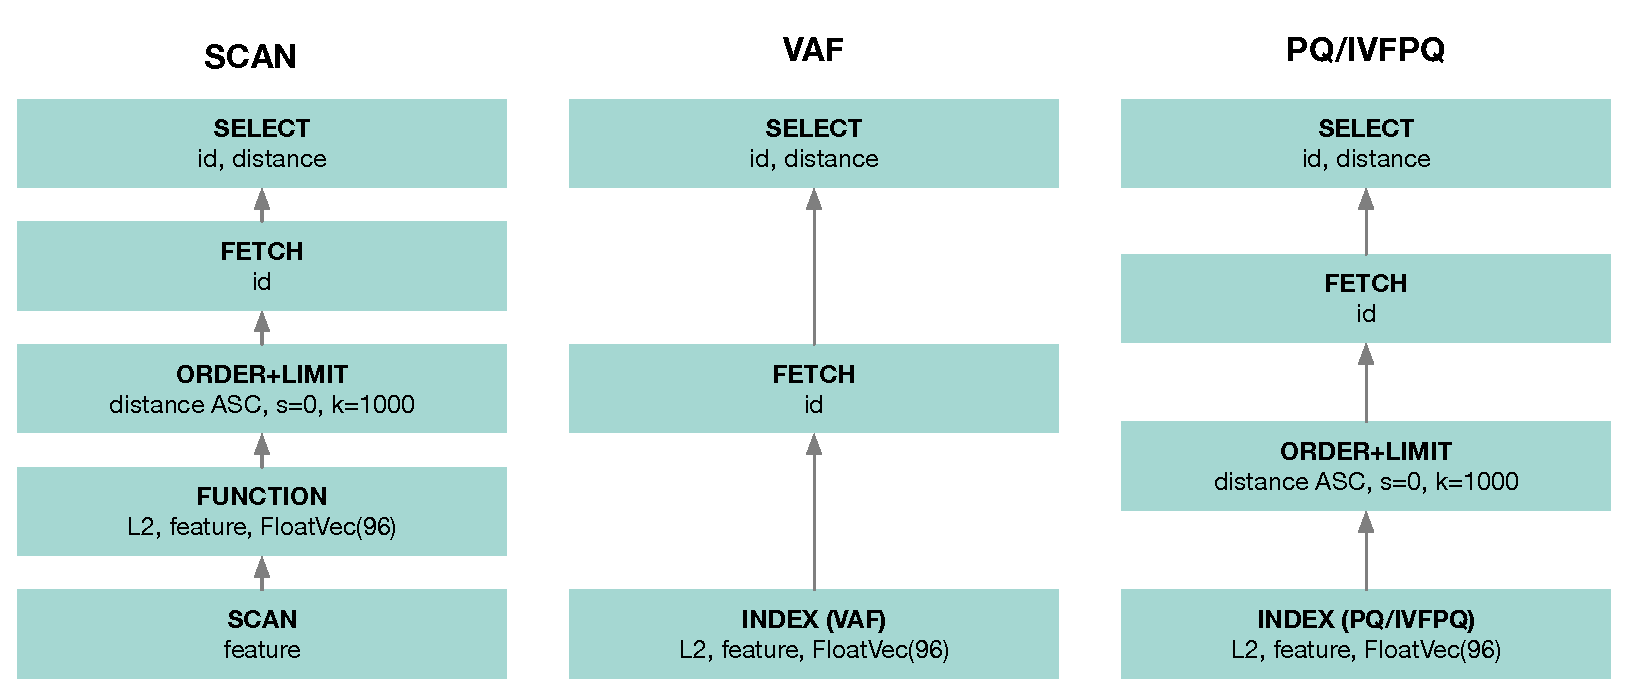
\includegraphics[width=\textwidth]{figures/bignns/cottontail/query-plan-nns}
        \caption{Simple \acrshort{nns}.}
        \label{figure:cottontail_nns_plan}
    \end{subfigure}
    \hfill
    \centering
    \begin{subfigure}[b]{\textwidth}
        \centering
        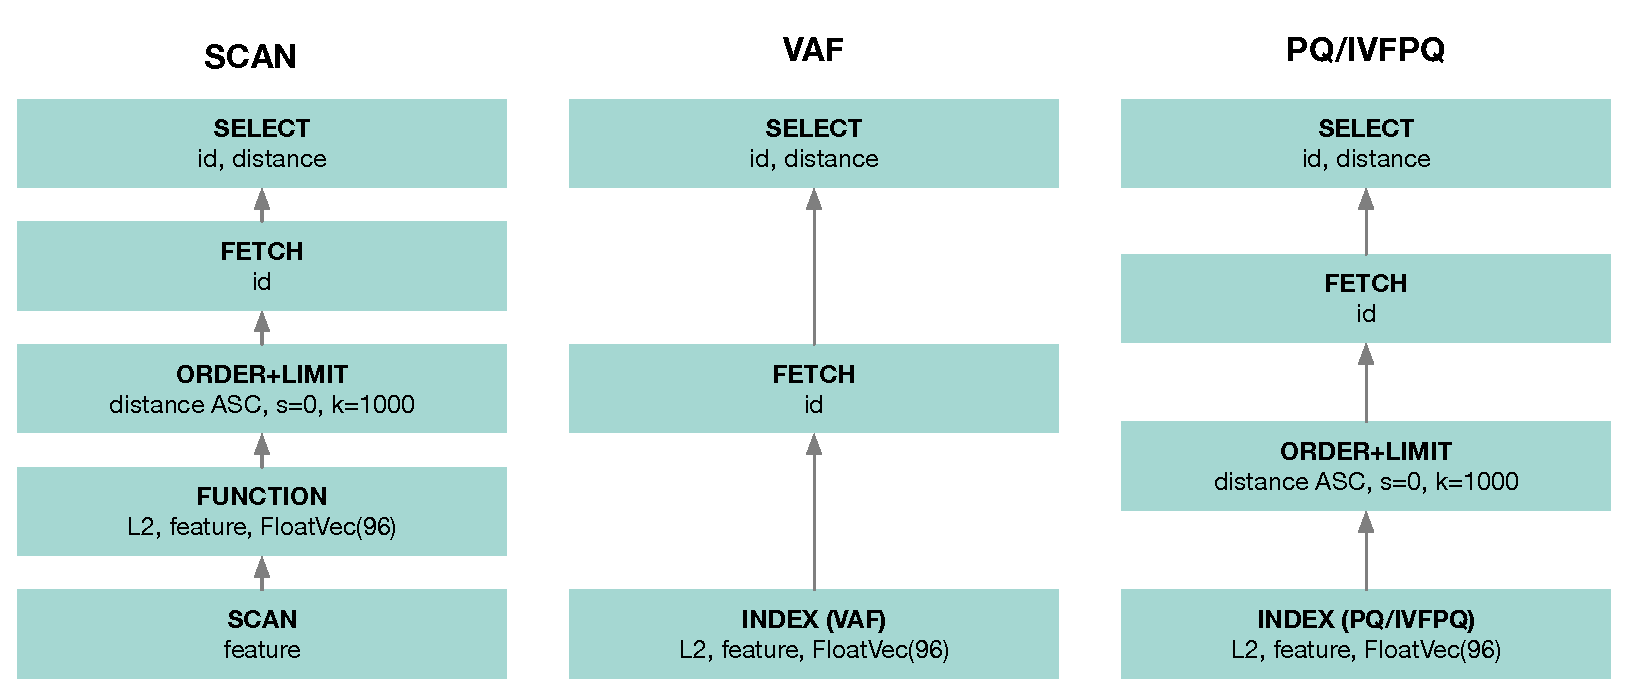
\includegraphics[width=\textwidth]{figures/bignns/cottontail/query-plan-nns}
        \caption{\acrshort{nns} and fetching of vectors.}
        \label{figure:cottontail_nns_fetch_plan}
    \end{subfigure}
    \hfill
    \centering
    \begin{subfigure}[b]{\textwidth}
        \centering
        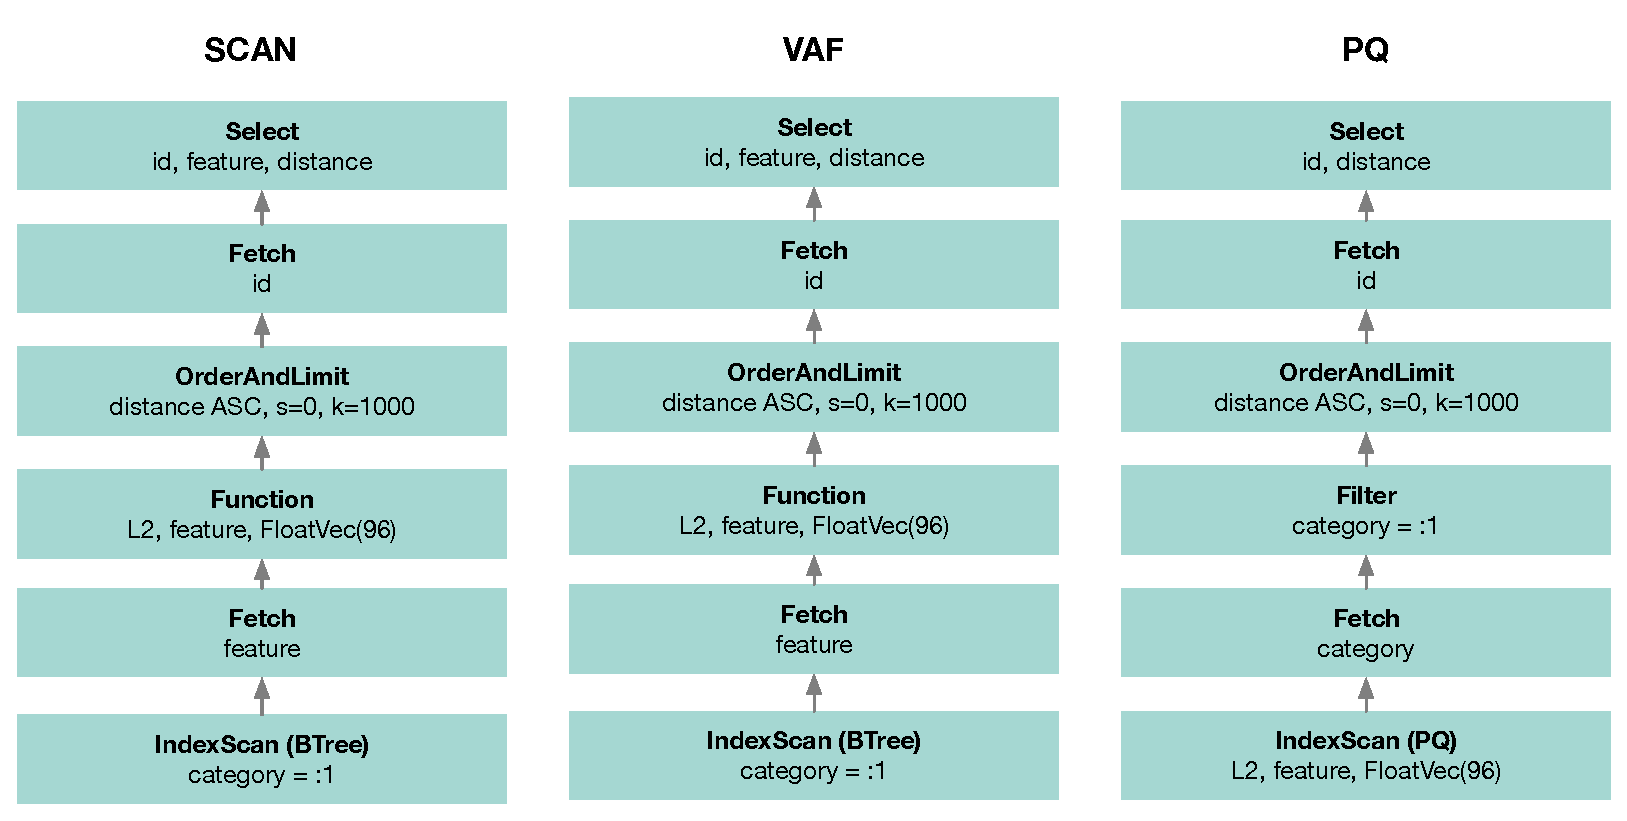
\includegraphics[width=\textwidth]{figures/bignns/cottontail/query-plan-hybrid}
        \caption{Hybrid query with Boolean filter.}
        \label{figure:cottontail_hybrid_plan}
    \end{subfigure}
    \caption{Execution plans produced by \cottontail{} for different query workloads prior to intra-query parallelisation. The use of the \acrshort{vaf} and \acrshort{pq} index was enforced using query hints.}
    \label{figure:cottontail_plans}
\end{figure}

Our second experiment involved the combined \acrshort{nns} and fetching of the resulting vectors. One can see in \Cref{figure:cottontail_nns_fetch_plan} that in terms of execution plan, accessing this additional column does not make a difference. Since both the plan involving the entity scan as well as the \acrshort{vaf} index scan produce the \texttt{feature} column early on, there is not need to fetch it later. Only for the \acrshort{pq} index -- which uses a distance approximation that is obtained without accessing the \texttt{feature} column -- an additional fetch is required. Consequently, the execution times are very similar to the simple \acrshort{nns} as one can see in \Cref{figure:cottontail_runtime} (NNS + Fetch). The numbers for a sequential scan range between $0.68 \pm 0.06 \, \si{\second}$ (5 million) and $344.08 \pm 8.02 \, \si{\second}$ (1 billion). The impact of the additional fetching of $1000$ feature columns is negligible for the \acrshort{pq} index, which can be attributed to the fact that the fetch is pushed until after the $s,k$-selection by the optimiser. We expect the impact of this fetching step to become more important for larger values of $k$ but it should remain negligible since typically, $k << N$. The quality metric shown in the appendix (\Cref{figure:appendix_bignns_cottontail_nns_fetch_quality}), are pretty much comparable to those of the first experiment, exhibiting the same, low numbers and high variance.

For the final experiment, we executed hybrid queries, i.e., \acrshort{nns} was restricted to a subset of the data that matches a Boolean predicate. The predicate involves a simple equality check that should effectively limit the exhaustive \acrshort{nns} to roughly $\frac{1}{10}$ of the collection. The values for a sequential scan range between $1.47 \pm 0.15 \, \si{\second}$ (5 million) and $349.66 \pm 7.0 \, \si{\second}$ (1 billion) with very similar numbers for the \acrshort{vaf} and \acrshort{pq} indexes. To make sense of these values, we again turn to the query plans illustrated in \Cref{figure:cottontail_runtime} (Hybrid). The sequential scan was executed with the help of a $B^{+}$-tree index, which speeds-up the Boolean filtering. Unfortunately, the current implementation of the \acrshort{vaf} index cannot natively accomodate Boolean predicates, since it constitutes a class 3 index replacement according to \Cref{definition:dfc_index_class_3} and therefore, a special implementation of the index would be required\footnote{It is, however, unclear if such an implementation would be beneficial in practice.}. Consequently, a $B^{+}$-tree scan was executed instead. In contrast, the \acrshort{pq} index can be combined with Boolean predicates, since it constitutes a class 1 index replacement according to \Cref{definition:dfc_index_class_1}. However, one can see in \Cref{figure:cottontail_runtime} (NNS + Fetch) that the advantage of using the \acrshort{pq} index is negligible.
This can be attributed to the fact that a fetch operation for the \texttt{category} column must be executed for every entry before executing the filtering. The IO overhead is much larger than the speed-up gained through the \acrshort{pq} index. This is confirmed by the numbers we see for the IVF\acrshort{pq} index, which restricts the scan to a small subset of the collection. Similarly to the IVF\acrshort{pq} index, the $B^{+}$-tree index does currently not allow for parallel evaluation due to \cottontail{}'s partitioning model. This is severly limiting for the hybrid queries and something that should be addressed in the future. The n\acrshort{dcg} and recall values are again shown in \Cref{chapter:appendix_results} (\Cref{figure:appendix_bignns_cottontail_hybrid_quality}).

In summary, all modes of operation fail to deliver interactive latency for very large collections, which currently is the price that must be paid for being bound to disk. It is to be noted, however, that \cottontail{} does not employ any caching other than a page cache. We presume that such advanced caching of, e.g., signatures could result in a considerable speed-up.

\subsection{Milvus}
For executing queries in Milvus, the mode of operation is a bit different than it is for \cottontail, since Milvus requires a data collection to be available in main memory, in order to be able to query it. Therefore, every query consists of two steps: Loading the collection and then executing the query once the collection is ready. We have obtained the ellapsed time for loading and query execution separately, so that we can reason about the individual components. The way queries can be specified is outlined in \Cref{listing:milvus_query}. We show the Python instead of the Java syntax, because it is less verbose and more readable, assuming, that the functionality of the two client libraries is identical.  

\begin{lstlisting}[language=Python, caption={Example of a similarity search query in a collection ``images'' using a 2-dimensional query vector and the Euclidean distance. Before executing the query, the data collection must be loaded.}, label=listing:milvus_query, numbers=none]
    from pymilvus import Collection
    
    # Load an existing collection.
    collection = Collection("images")      
    collection.load()

    # Perform search.
    query = [[0.0, 0.0]]
    params = {"metric_type": "L2", "params": {"nprobe": 10}}
    results = collection.search(
        data=query, anns_field="feature", param=params, limit=10
    )
\end{lstlisting}

Accross all workloads, we compared the performance of two different types of indexes: The \texttt{FLAT} index is the equivalent of a sequential scan and it is the only index in Milvus that guarantees a recall of $1.0$. The \texttt{IVF\_SQ8} index uses an inverted file of clusters and limits search to a subset of these clusters based on the parameters provided by the user and an initial distance calculation between the query and the cluster centers. The approach is comparable to cluster pruning \cite{Chierichetti:2007Finding} or the two stage quantisation process described in \cite{Jegou:2010Product}, where each vector is mapped to an inverted list using a coarse quantiser. In addition to limiting the search space, the \texttt{IVF\_SQ8} index also compresses the \SI{4}{\byte} (\texttt{float}) into a \SI{1}{\byte} (\texttt{int8}) presentation, which significantly reduces memory and \acrshort{cpu} usage by up to 70\%. We built the \texttt{IVF\_SQ8} index beforehand using $4096$ clusters and instructed Milvus to consider $1024$ and $2048$ (query parameter \texttt{nprobe}) clusters respectively, when searching the collection.

\begin{landscape}
    \begin{figure}[p]
        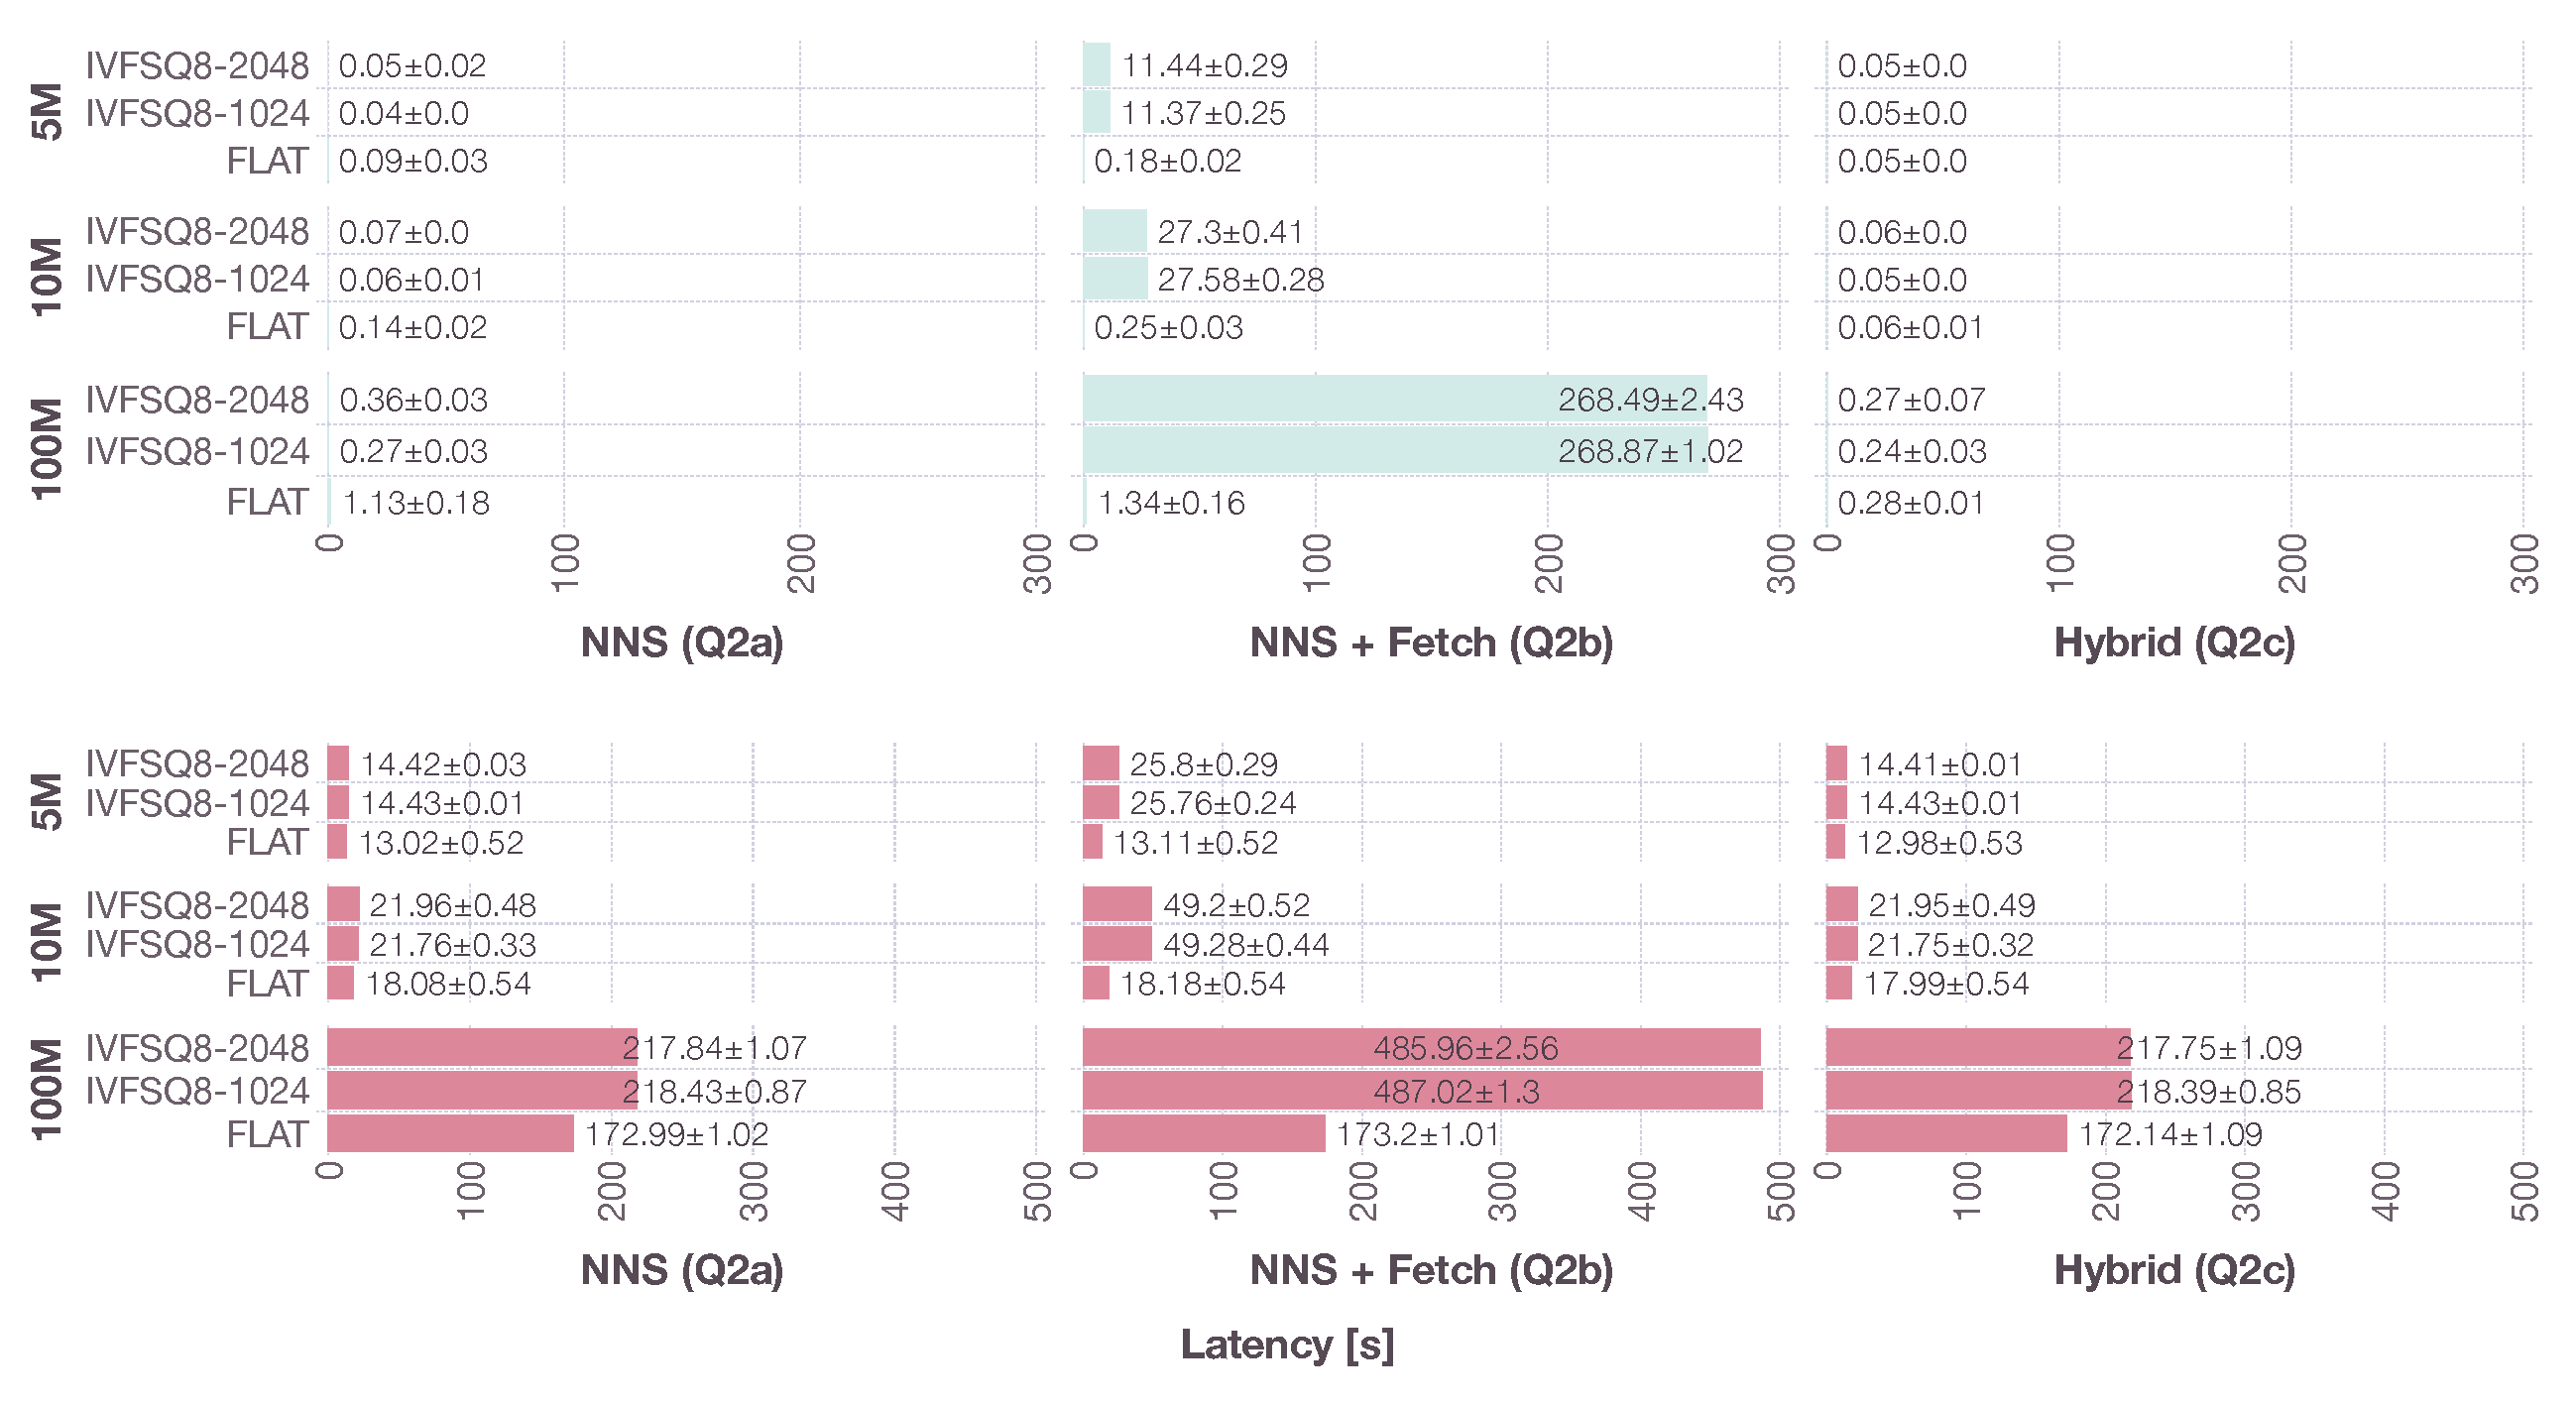
\includegraphics[width=1.6\textwidth]{figures/bignns/milvus/bignns-milvus}
        \caption{Milvus's latency in seconds for different workloads (x-axis) on different shards of the Deep 1B data set using different access methods (y-axis), with (red) and without (mint) time used for loading the data from disk.}
        \label{figure:milvus_runtime}
    \end{figure}
\end{landscape}

In our first experiment we executed the simple \acrshort{nns} workload (Q2a). The results are depicted in Figure \Cref{figure:milvus_runtime}. We can summarise that even for brute-force search (\texttt{FLAT}), query execution speed is very impressive once a collection has been loaded into main memory. For our test collection, it took between $0.09 \pm 0.03 \, \si{\second}$ (5 million) and $1.3 \pm 0.18 \, \si{\second}$ (100 million) to execute a query, all the while retaining a perfect recall and \acrshort{dcg} of $1.0$. However, if one considers time required to load a collection from disk to be part of the query time, these numbers rise to between $13.02 \pm 0.52 \, \si{\second}$ and $172.99 \pm 1.02 \, \si{\second}$. If one loads a collection once to then execute many queries thereafter, the performance provided by Milvus is very desirable as the cost of loading the collection can be amortised over time. However, if a large number of collections must be queried without the ability to predict which one, and not all collections can be pre-loaded, query exection time is expected to deteriorate. Furthermore, the requirement to load the collection prior to querying it turned out to be an insurmountable roadblock for the shard that contained 1 billion entries. Milvus was unable to load the collection as it ran out of available memory. We can confirm, that Milvus indeed used-up the entire \SI{376}{\giga\byte} of \acrshort{ram} available on the node.

In an attempt to aleviate the memory pressure, we also considered the \texttt{IVF\_SQ8} index, which seems a logical choice due to its data compression characteristics. Unfortunately, using this index instead did not resolve the problem of collection loading, since apparently, Milvus always loads the indexes and the raw data. Nevertheless, there are two interesting insights from the data we gathered:
\begin{enumerate*}[label=(\roman*)]
    \item \texttt{IVF\_SQ8} brings considerable speed-up for raw query execution time, especially for larger collections (roughly \SI{1}{\second} faster on 100 million shard),
    \item however, it exacerbates the performance impact of collection loading, since the indexes must apparently be loaded in addition to the raw data.
\end{enumerate*}

The experiment involved the combined \acrshort{nns} and fetching of the resulting vectors. Unfortuntely, Milvus currently doesn't support the returning of vectors in a \acrshort{nns}, which is why this is a two-step process. First, the \acrshort{nns} is executed. Then the vectors for the resulting primary key's must be fetched. We measure the time for both steps but do not reload the collection in between. The results are depicted in \Cref{figure:milvus_runtime} (Q2b). The additional fetching step, while cumbersome, does not seem to have a negative impact in cases where the \texttt{FLAT} index is used. However, use of the \texttt{IVF\_SQ8} index seems to lead to significant deterioration of the the query performance for the fetching step, adding approximately \SI{10}{\second} (5 million) to more than \SI{250}{\second} (100 million) to query execution time. We do not have an explanation for this and consider this to be abnormal behaviour.

Last but not least, we did execute hybrid queries, wherein \acrshort{nns} was restricted to a subset of the data that was filtered by a simple predicate. In Milvus, this is a query primitive that is part of the similarity search \acrshort{api}. The results are visualised in \Cref{figure:milvus_runtime} (Q2c) and do not hold any surprises. In-memory query execution speed is again outstanding whereas time required to load a collection is significant. Interestingly, the \texttt{IVF\_SQ8} did not seem to have a negative impact on query execution speed, which confirms our suspicion that the deterioration observed in the second experiment must be considered a bug.

We refrain from visualising n\acrshort{dcg} and recall values but can report that recall was always $1.0$ for \texttt{FLAT} and around $0.99$ for all queries that used the \texttt{IVF\_SQ8} index.

\subsubsection{Qualitative Assesment}
While very convincing in terms of sheer execution speed, the current version of Milvus also has some limitations that we list here for future reference:

\begin{itemize}
    \item Milvus currently only supports the Euclidean and Inner Product distance for \acrshort{nns} on floating point embeddings. There is no way to use other metrics. It therefore doesn't offer the flexibility of \cottontail{}.
    \item Milvus does not support proximity-based search strategies other than \acrshort{nns} and again lacks the flexibility of \cottontail{}. However, according to the official GitHub issue tracker, \footnote{See https://github.com/milvus-io/milvus/issues/17599/, Accessed August 2022} range search is due for the 2.2.0 release. 
    \item Milvus cannot retrieve the feature vectors as part of a \acrshort{nns}, i.e., they must be fetched in an additional query by looking them up based on the primary key. This issue is also due for being addressed in the 2.2.0 release. \footnote{See https://github.com/milvus-io/milvus/issues/16538/, Accessed August 2022}
    \item Milvus can only maintain a single index per feature column. This effectively limits the set of available distance functions to one, since most indexes must be trained for a specific distance.
\end{itemize}

In addition, we have observed that as Milvus uses up all the memory during collection loading, it starts to (mis-)behave eraticly making it difficult to unload the collection again. In some of our runs, it started to reload the same collection after a restart, effectively rendering the entire instance unusable for several hours.

\section{High-Dimensional Index Maintenance}
\label{section:hd_index_maintenance_evaluation}

With this evaluation, we demonstrate \cottontail{}'s ability to cope with data that is subject to constant change. It is a test of the high-dimensional index maintenance mechanism described in \Cref{section:hd_index_maintenance}. The setup of this experiment is slightly different than that of all previous experiments, in that it involves different workloads that run concurrently: The benchmark starts by creating an entity and loading it with $1$ million entries -- we again use the Yandex Deep 1B ($d = 96$) dataset as a basis here. After data loading has completed, we generate and build an index -- either a \acrshort{vaf} ($35$ marks per vector component) or a \acrshort{pq} index ($8$ subspaces, $2048$ centroids). Once the entity is ready, the actual measurements start. We run two threads is parallel -- on thread randomly inserts new data from the Yandex Deep 1B dataset or it deletes data points (we use a 90\%, 10\% mix for inserts and deletes). The other thread continuously executes \acrshort{nns} queries, once using the previously created index and once employing a brute-force scan to obtain the groundtruth. We run this experiment over the course of \SI{1}{\hour} and observe how the collection itself, the latency of the \acrshort{nns} queries and the quality of the results develops over time.

\section{Summary and Discussion}
\label{section:discussion}

With this evaluation, we have demonstrated the applicability of the concepts introduced in \Cref{chapter:system_model} to practical scenarios. The notion of generalised, proximity based operations as an extension to the relation algebra described in \Cref{section:generalised_proximity_based_ops} provide us with the ability to construct and execute a wide range of query workloads in a much more flexible way then purpose built systems such as Milvus \cite{Wang:2021Milvus} can provide. Furthermore, the proposed algebra enables the \acrshort{dbms} to decompose and optimise queries based on the needs expressed by a system user and the parameters of the system itself. 

While our reference implementation \cottontail{} may not be able to compete in terms of raw processing speed, it still seems to do pretty well against Milvus when loading data from disk is considered as well. In our experiments, during the time that Milvus required to load a collection, \cottontail{} could query the same collection between $15$ (VAF) to $34$ (PQ) times, all the while retaining the flexibility to switch between collections and/or execute different types of workloads. Maintaining and accessing all the relevant data on disk incurs an overhead that makes it difficult or even impossible to reach the processing speed of with in-memory systems. This has been pointed out my L. Amsaleg, who stated that ``When purposely dealing with secondary storage, it is hard if not impossible to beat high-dimensional indexing solutions that have been designed to run in main memory. This is unfortunately true even for collections that might fit in main memory, as enforcing durability etc. generates a substantial overhead.'' (\cite{Amsaleg:2014Database}, p. 12). Yet, the experiments have also demonstrated the limitations of pure in-memory processing in cases where collections simply do not fit into main memory.

\subsection{Generalised Proximity Based Queries}

Over the years, many information retrieval models \cite{Umano:1983Retrieval,Salton:1983Extended,Wong:1985Generalized} have been proposed. Some of these models are mainly set-based \cite{Salton:1983Extended,Umano:1983Retrieval}, and thus similar to the relational model \cite{Codd:1970Relational}, while others are based entirely on the vector space model that considers documents to be high-dimensional vectors \cite{Wong:1985Generalized}. Our approach uses the relational model as a foundation and integrates the notion of complex data types (e.g., vectors), scoring and ranking as explicit extensions. In that it follows a tradition of extending the expressive power of \acrshort{sql} and the relational model \cite{Libkin:2003Expressive}, that has been practiced for many years \cite{Chengkai:2005RankSQL,Zhang:2006Boolean,Belohlavek:2007Relational}, as we have argued in \Cref{section:rel_extensions}. Conceptually, we see the proposed extensions as a first, minimally invasive step towards the realisation of the \cite{Extended Boolean Retrieval Model} as proposed in \cite{Salton:1983Extended}. In such a model, distances and scores can be employed to perform advanced operations such as fuzzy-set operations or similarity joins \cite{Umano:1983Retrieval,Zadeh:1996Fuzzy,Bohm:2001Fast}. From our perspective and with an eye on analytics workloads, we would add primitives such a clustering or \acrshort{rnns} to that list as well.

The convergence of information retrieval and databases as well as the addition of multimedia support have been a reocurring subject at many of the database self-assessment meetings since the 1980s \cite{Agrawal:2008Claremont}. Unsurprisingly, many approaches at convergence have been attempted over the years at a conceptual \cite{Marcus:1996Foundations,Adjeroh:1997Multimedia,Watanabe:1998Multimedia}, logical \cite{Zhang:2006Boolean,Belohlavek:2007Relational} and physical level \cite{Silva:2010SimDB,Giangreco:2014Adam,Giangreco:2016Adam,Yang:2020Pase}. The model we propose provides a sound, theoretical foundation rooted in relational algebra and has been demonstrated to be useful in practical scenarios, both experimental \cite{Boerlin:20203d} and simple \cite{Rossetto2019:Retrieval,Sauter2020:Combining,Heller:2021Towards}. An important, mental step that enables such a simple yet expressive model is that of ``separation of concerns'', as proposed by \cite{Giangreco:2018Database} and in fact realised in the entire \vitrivr{} ecosystem \cite{Rossetto:2016Vitrivr,Gasser:2019Multimodal}. While similarity search and retrival may be the end goal, from a database perspective, we merely execute simple primitives such as evaluation of functions, sorting and selection going in a similar direction as systems such SciDB \cite{Stonebraker:2013SciDB} and Monet DB \cite{Idreos:2012MonetDB}, that mainly provide support for analytical workloads. By carefully ignoring the noise introduced by higher-level concepts such as documents, segments, features, scores and distances -- which may not be useful for data processing -- the database system can focus on its core purpose which is that of providing reliable and fast data management and access and leave the advanced data modelling to upper-tier system components.

Since \adampro \cite{Giangreco:2016Adam} is \cottontail{}'s predecessor and one of the inspirations for the work presented in this Thesis, we would also like to higlight the differences between the query model proposed in \cite{Giangreco:2018Database} and our own. While \cite{Giangreco:2018Database} postulates the existence of a similarity operator -- which works similarily to our extended projection -- it merely uses it to derive more restricted versions that basically consider \acrshort{nns} and range search (\epsilon NN) to be dedicated query primitives. While simple to implement and test, the approach is demonstrably limited in the types of queries it can accomodate. Moreover, it introduces logical flaws, e.g., the question of operator precedence when combining Boolean and similarity based selection. Nevertheless, other systems, such as Milvus \cite{Wang:2021Milvus}, take a similar approach as they add query primitives for the different types of workloads they accomodate - leading to growing number of disjoint APIs for different purposes. We don't consider this a sustainable approach, since it ignores future workloads that may combine existing primitives in a different way (e.g., aggregating on distance or \acrshort{fns}). Furthermore, generating specialised blackbox operators for different types of high-level primitives, limits the potential for optimisation by the \acrshort{dbms}. 

\cite{Giangreco:2018Database} also considers the distance or score to be an implicit attribute introduced by the proposed similarity operations, wheras we use the extended projection to make it explicit. While this may seem like a finer point of semantics at first, we argue, that making the attribute explicit is what allows downstream processing such as normalisation (from distance to score), combination of multiple distances (or scores) to express score fusion and any variant thereof \cite{Bohm:2001Fast}. Ultimately, we consider it to be at the discretion of the user to decide whether calculated attributes should be used and included and the task of the query optimiser to take these decisions into account when preparing an efficient execution plan.

In contrast to \cite{Giangreco:2018Database}, the relational algebra extensions we propose are rather limited and lie well within the capabilities most modern \acrshort{dbms} bring today. In line with \Cref{Abadi:2014Beckman,Abadi:2020Seattle}, we identify the efficient execution of the functions (or linear algebra, for that matter) involved using the different means in terms of hard- and software, as important, future research directions. In addition to execution models that consider special hardware such as \acrshort{simd} instructions or \acrshort{gpu}s, we also believe the relationship between such functions and (approximate) indexing techniques to be promising avenues to explore. In order to be able to do so, these functions must be enriched with metainformation that allows for optimisation at different levels of the query execution engine.

\subsection{Query Planning and Cost Model}  
In \Cref{section:cost_model} we have proposed a cost model that takes the expected quality of results into account and we have discussed methods that can be used to estimate that quality for different, known query plans. Our reference implementation \cottontail{} uses a query planner that leverages the aforementioned cost-model to determine the optimal execution path given a query and a cost policy specified by the user, as demonstrated in \Cref{section:cost_model_evaluation}.

To the best of our knowledge, both aspects -- the estimation of qualtiy as well as its use in a cost model for query planning -- are rather uncommon today. Even though the quality vs. execution time trade-off is an implicit consequence of approximate solutions to proximity-based search in general and \acrshort{nns} in particular, there is very little research that considers this issue systematically, with a few, notable exceptions \cite{Weber:2000Trading,Blok2001:Predicting,Siguroardottir:2005Quality}. This is reflected by the fact, that most state-of-the-art approximate index structures fail to provide any strong quality guarantees \cite{Echihabi:2021High}. Here we see a huge corpus for future research: On the one hand, we see a need for index structures that provide explicit quality guarantees such as \cite{Lu:2020VHP}. On other hand, we should explore system-level mechanisms that continuously evaluate the efficiency and effectivenes by which results have been produced and adjust the cost model accordingly. This has already been proposed by \cite{Giangreco:2018Database}. The cost-model we propose can be seen as a foundation for such a continuous control loop between the query execution engine and the query planner.

\subsection{High-Dimensional Index Maintenance}

Maintaining a durable and consistent state and providing transactional guarantees for data structures required to execute queries -- including secondary index structures -- is a basic trait shared by most if not all traditional \acrshort{sql} and NoSQL systems. For some reason, however, durability and the notion of isolation and consistency in the face of dynamic data are aspects often overlooked for high-dimensional indexing \cite{Amsaleg:2014Database,Hojsgaard:2019Index}, especially in combination \cite{Amsaleg:2014Database}. In \Cref{section:hd_index_maintenance}, we have proposed a system-level mechanism for maintaining high-dimensional index structures on disk and for processing online changes to the data. The viability of the proposed mechanism was demonstrated in \Cref{section:hd_index_maintenance_evaluation}, based on two concrete examples.

Despite a large corpus of reasearch that dates back to the 70s \cite{Bentley:1975Multidimensional,Guttmann:1984RTrees,Beckmann:1990RTree,Indyk1998:Approximate,Weber:1998Va,Jegou:2010Product}, high-dimensional indexing for \acrshort{nns} and \acrshort{anns} is still a very relevant topic today \cite{Shimomura:2021Survey,Kraska:2018Case}, with more recent, graph-based methods showing a lot of promise. Since different index structures provide different properties in terms of scalability, performance and quality (guarantees) and can potentially be employed for different tasks, we regard this work as pivotal for further extending the indexing capabilities of multimedia \acrshort{dbms}. Many of these indexes can be seen as potential extensions to systems like \cottontail{} and should be investigated with regards to their write- and failure model.

The topic of disk-based \acrshort{anns} has been getting more attention lately, with emerging techniques such as DiskANN \cite{Jayaram:2019DiskANN} or SPANN \cite{Chen:2021SPANN}, which both advertise a hybrid in-memory/on-disk model and report impressive numbers for both latency and recall. Howver, both these state-of-the-art algorithms do not consider dynamic data at all and operate on the premise that the complete data collection must be (re-)indexed. Nevertheless, such efforts lay important groundwork for disk-based multimedia index maintenance and should and could be extended in terms of their ability to process incremental changes.

In \cite{Lejsek:2011NVTree,Lejsek:2009NVTree}, the authors propose the NV-tree, which is a disk-resident, high-dimensional index structure that provides transactional support \cite{Lejsek:2018Transactional}. The NV-tree would make a great extension to \cottontail{} and we expect it to fully fit into the proposed model for index maintainence in that it is an index structure that does not fail per-se and should not exhibit deterioration due to dynamic data. However, unfortunately the index structure itself seems proprietary and the available literature does not provide us with enough information to come up with out own implementation.

The subject of online indexing has also been addressed by some authors, for cases such as \acrshort{pq} \cite{Xu:2018Online}, \acrshort{lsh} \cite{Cakir:2015Adaptive} or graph-based methods \cite{Zhao:2022Approximate}. These are important contributions towards a write-model for different types of indexing techniques. However, the proposed methods lack a notion of index state and transactionality and they do not consider indexes to be durable data structures.

We have also highlighted different vector database systems in \Cref{section:vector_databases}, which all somehow face the issue of dynamic data: Milvus \cite{Wang:2021Milvus} handles inserts by marking them with timestamps and it allows for configurable consistency levels that differ in the timestamps of entries that are being considered. Hence, it uses a kind of \acrshort{mvcc}-based consistency and concurrency control model, similarly to \cottontail. Deletes are enabled by setting bit mask for deleted entries and filtering them on the fly at query time. However, for both mechanisms, it is not fully clear how they scale as changes accumulate. Nevertheless, some concepts employed by Milvus may be very interesting, e.g., the (re-)indexing of chunks rather than the entire data collection at once. Vald \footnote{See https://github.com/vdaas/vald/, Accessed August 2022} advertises a ``asynchronous auto indexing'' that uses ``distributed index graphs'' to avoid locking the entire graph during indexing. However, it is not clear what type of guarantees are provided by this mechanism other than preventing a system-wide halt. Unfortunately, for Qdrant \footnote{See https://github.com/qdrant/qdrant/, Accessed July 2022} , we could not find any information as to how dynamic data and concurrency is handled.

